\documentclass{article}

% packages
  % basic stuff for rendering math
  \usepackage[letterpaper, top=1in, bottom=1in, left=1in, right=1in]{geometry}
  \usepackage[utf8]{inputenc}
  \usepackage[english]{babel}
  \usepackage{amsmath} 
  \usepackage{amssymb}
  % \usepackage{amsthm}

  % extra math symbols and utilities
  \usepackage{mathtools}        % for extra stuff like \coloneqq
  \usepackage{mathrsfs}         % for extra stuff like \mathsrc{}
  \usepackage{centernot}        % for the centernot arrow 
  \usepackage{bm}               % for better boldsymbol/mathbf 
  \usepackage{enumitem}         % better control over enumerate, itemize
  \usepackage{hyperref}         % for hypertext linking
  \usepackage{fancyvrb}          % for better verbatim environments
  \usepackage{newverbs}         % for texttt{}
  \usepackage{xcolor}           % for colored text 
  \usepackage{listings}         % to include code
  \usepackage{lstautogobble}    % helper package for code
  \usepackage{parcolumns}       % for side by side columns for two column code
  \usepackage{array} 

  % page layout
  \usepackage{fancyhdr}         % for headers and footers 
  \usepackage{lastpage}         % to include last page number in footer 
  \usepackage{parskip}          % for no indentation and space between paragraphs    
  \usepackage[T1]{fontenc}      % to include \textbackslash
  \usepackage{footnote}
  \usepackage{etoolbox}
  \usepackage[table]{xcolor}

  % for custom environments
  \usepackage{tcolorbox}        % for better colored boxes in custom environments
  \tcbuselibrary{breakable}     % to allow tcolorboxes to break across pages

  % figures
  \usepackage{pgfplots}
  \pgfplotsset{compat=1.18}
  \usepackage{float}            % for [H] figure placement
  \usepackage{tikz}
  \usepackage{tikz-cd}
  \usepackage{circuitikz}
  \usetikzlibrary{shapes,arrows,positioning}
  \usetikzlibrary{arrows}
  \usetikzlibrary{positioning}
  \usetikzlibrary{calc}
  \usepackage{graphicx}
  \usepackage{caption} 
  \usepackage{subcaption}
  \captionsetup{font=small}

  % for tabular stuff 
  \usepackage{dcolumn}

  \usepackage[nottoc]{tocbibind}
  \pdfsuppresswarningpagegroup=1
  \hfuzz=5.002pt                % ignore overfull hbox badness warnings below this limit

% New and replaced operators
  \DeclareMathOperator{\Tr}{Tr}
  \DeclareMathOperator{\Sym}{Sym}
  \DeclareMathOperator{\Span}{span}
  \DeclareMathOperator{\std}{std}
  \DeclareMathOperator{\Cov}{Cov}
  \DeclareMathOperator{\Var}{Var}
  \DeclareMathOperator{\Corr}{Corr}
  \DeclareMathOperator{\pos}{pos}
  \DeclareMathOperator*{\argmin}{\arg\!\min}
  \DeclareMathOperator*{\argmax}{\arg\!\max}
  \newcommand{\ket}[1]{\ensuremath{\left|#1\right\rangle}}
  \newcommand{\bra}[1]{\ensuremath{\left\langle#1\right|}}
  \newcommand{\braket}[2]{\langle #1 | #2 \rangle}
  \newcommand{\qed}{\hfill$\blacksquare$}     % I like QED squares to be black
  \def\ojoin{\setbox0=\hbox{$\bowtie$}%
    \rule[-.02ex]{.25em}{.4pt}\llap{\rule[\ht0]{.25em}{.4pt}}}
  \def\lojoin{\mathbin{\ojoin\mkern-5.8mu\bowtie}}
  \def\rojoin{\mathbin{\bowtie\mkern-5.8mu\ojoin}}
  \def\fojoin{\mathbin{\ojoin\mkern-5.8mu\bowtie\mkern-5.8mu\ojoin}}
% Custom Environments
  \newtcolorbox[auto counter, number within=section]{question}[1][]
  {
    colframe = orange!25,
    colback  = orange!10,
    coltitle = orange!20!black,  
    breakable, 
    title = \textbf{Question \thetcbcounter ~(#1)}
  }

  \newtcolorbox[auto counter, number within=section]{exercise}[1][]
  {
    colframe = teal!25,
    colback  = teal!10,
    coltitle = teal!20!black,  
    breakable, 
    title = \textbf{Exercise \thetcbcounter ~(#1)}
  }
  \newtcolorbox[auto counter, number within=section]{solution}[1][]
  {
    colframe = violet!25,
    colback  = violet!10,
    coltitle = violet!20!black,  
    breakable, 
    title = \textbf{Solution \thetcbcounter}
  }
  \newtcolorbox[auto counter, number within=section]{lemma}[1][]
  {
    colframe = red!25,
    colback  = red!10,
    coltitle = red!20!black,  
    breakable, 
    title = \textbf{Lemma \thetcbcounter ~(#1)}
  }
  \newtcolorbox[auto counter, number within=section]{theorem}[1][]
  {
    colframe = red!25,
    colback  = red!10,
    coltitle = red!20!black,  
    breakable, 
    title = \textbf{Theorem \thetcbcounter ~(#1)}
  } 
  \newtcolorbox[auto counter, number within=section]{proposition}[1][]
  {
    colframe = red!25,
    colback  = red!10,
    coltitle = red!20!black,  
    breakable, 
    title = \textbf{Proposition \thetcbcounter ~(#1)}
  } 
  \newtcolorbox[auto counter, number within=section]{corollary}[1][]
  {
    colframe = red!25,
    colback  = red!10,
    coltitle = red!20!black,  
    breakable, 
    title = \textbf{Corollary \thetcbcounter ~(#1)}
  } 
  \newtcolorbox[auto counter, number within=section]{proof}[1][]
  {
    colframe = orange!25,
    colback  = orange!10,
    coltitle = orange!20!black,  
    breakable, 
    title = \textbf{Proof. }
  } 
  \newtcolorbox[auto counter, number within=section]{definition}[1][]
  {
    colframe = yellow!25,
    colback  = yellow!10,
    coltitle = yellow!20!black,  
    breakable, 
    title = \textbf{Definition \thetcbcounter ~(#1)}
  } 
  \newtcolorbox[auto counter, number within=section]{example}[1][]
  {
    colframe = blue!25,
    colback  = blue!10,
    coltitle = blue!20!black,  
    breakable, 
    title = \textbf{Example \thetcbcounter ~(#1)}
  } 
  \newtcolorbox[auto counter, number within=section]{code}[1][]
  {
    colframe = green!25,
    colback  = green!10,
    coltitle = green!20!black,  
    breakable, 
    title = \textbf{Code \thetcbcounter ~(#1)}
  } 

  \BeforeBeginEnvironment{example}{\savenotes}
  \AfterEndEnvironment{example}{\spewnotes}
  \BeforeBeginEnvironment{lemma}{\savenotes}
  \AfterEndEnvironment{lemma}{\spewnotes}
  \BeforeBeginEnvironment{theorem}{\savenotes}
  \AfterEndEnvironment{theorem}{\spewnotes}
  \BeforeBeginEnvironment{corollary}{\savenotes}
  \AfterEndEnvironment{corollary}{\spewnotes}
  \BeforeBeginEnvironment{proposition}{\savenotes}
  \AfterEndEnvironment{proposition}{\spewnotes}
  \BeforeBeginEnvironment{definition}{\savenotes}
  \AfterEndEnvironment{definition}{\spewnotes}
  \BeforeBeginEnvironment{exercise}{\savenotes}
  \AfterEndEnvironment{exercise}{\spewnotes}
  \BeforeBeginEnvironment{proof}{\savenotes}
  \AfterEndEnvironment{proof}{\spewnotes}
  \BeforeBeginEnvironment{solution}{\savenotes}
  \AfterEndEnvironment{solution}{\spewnotes}
  \BeforeBeginEnvironment{question}{\savenotes}
  \AfterEndEnvironment{question}{\spewnotes}
  \BeforeBeginEnvironment{code}{\savenotes}
  \AfterEndEnvironment{code}{\spewnotes}

  \definecolor{dkgreen}{rgb}{0,0.6,0}
  \definecolor{gray}{rgb}{0.5,0.5,0.5}
  \definecolor{mauve}{rgb}{0.58,0,0.82}
  \definecolor{lightgray}{gray}{0.93}

  % default options for listings (for code)
  \lstset{
    autogobble,
    frame=ltbr,
    language=SQL,                           % the language of the code
    aboveskip=3mm,
    belowskip=3mm,
    showstringspaces=false,
    columns=fullflexible,
    keepspaces=true,
    basicstyle={\small\ttfamily},
    numbers=left,
    firstnumber=1,                        % start line number at 1
    numberstyle=\tiny\color{gray},
    keywordstyle=\color{blue},
    commentstyle=\color{dkgreen},
    stringstyle=\color{mauve},
    backgroundcolor=\color{lightgray}, 
    breaklines=true,                      % break lines
    breakatwhitespace=true,
    tabsize=3, 
    xleftmargin=2em, 
    framexleftmargin=1.5em, 
    stepnumber=1
  }

% Page style
  \pagestyle{fancy}
  \fancyhead[L]{Databases}
  \fancyhead[C]{Muchang Bahng}
  \fancyhead[R]{Fall 2024} 
  \fancyfoot[C]{\thepage / \pageref{LastPage}}
  \renewcommand{\footrulewidth}{0.4pt}          % the footer line should be 0.4pt wide
  \renewcommand{\thispagestyle}[1]{}  % needed to include headers in title page

\begin{document}

\title{Databases}
\author{Muchang Bahng}
\date{Fall 2024}

\maketitle
\tableofcontents
\pagebreak

  This is a course on database languages (SQL), database systems (Postgres, SQL server, Oracle, MongoDB), and data analysis. 

  \begin{definition}[Data Model]
    A \textbf{data model} is a notation for describing data or information, consisting of 3 parts. 
    \begin{enumerate}
      \item \textit{Structure of the data}. The physical structure (e.g. arrays are contiguous bytes of memory or hashmaps use hashing). This is higher level than simple data structures. 
      \item \textit{Operations on the data}. Usually anything that can be programmed, such as \textbf{querying} (operations that retrieve information), \textbf{modifying} (changing the database), or \textbf{adding/deleting}. 
      \item \textit{Constraints on the data}. Describing what the limitations on the data can be. 
    \end{enumerate}
  \end{definition}

  There are two general types: relational databases, which are like tables, and semi-structured data models, which follow more of a tree or graph structure (e.g. JSON, XML).  

\section{Relational Algebra}

  The most intuitive way to store data is with a \textit{table}, which is called a relational data model, which is the norm since the 1990s. 

  \begin{definition}[Relational Data Model]
    A \textbf{relational data model} is a data model where its structure consists of 
    \begin{enumerate}
      \item \textbf{relations}, which are two-dimensional tables. 
      \item Each relation has a set of \textbf{attributes}, or columns, which consists of a name and the data type (e.g. int, float, string, which must be primitive).\footnote{The attribute type cannot be a nonprimitive type, such as a list or a set. }
      \item Each relation is a set\footnote{Note that since this is a set, the ordering of the rows doesn't matter , even though the output is always in some order.} of \textbf{tuples} (rows), which each tuple having a value for each attribute of the relation. Duplicate (agreeing on all attributes) tuples are not allowed. 
    \end{enumerate}
    So really, relations are tables, tuples are rows, attributes are columns. 
  \end{definition}

  \begin{definition}[Schema]
    The \textbf{schema} of a relational database just describes the form of the database, with the name of the database followed by the attributes and its types. 
    \begin{lstlisting}
      Beer (name string, brewer string)
      Serves (bar string, price float)
      ...
    \end{lstlisting}
  \end{definition}

  \begin{definition}[Instance]
    The entire set of tuples for a relation is called an \textbf{instance} of that relation. If a database only keeps track of the instance now, the instance is called the \textbf{current instance}, and \textbf{temporal databases} also keep track of the history of its instances. 
  \end{definition}

  SQL (Structured Query Language) is the standard query language supported by most DBMS. It is \textbf{declarative}, where the programmer specifies what answers a query should return,but not how the query should be executed. The DBMS picks the best execution strategy based on availability of indices, data/workload characteristics, etc. (i.e. provides physical data independence). It contrasts to a \textbf{procedural} or an \textbf{operational} language like C++ or Python. One thing to note is that keywords are usually written in uppercase by convention. 

  \begin{definition}[Primitive Types]
    The primitive types are listed. 
    \begin{enumerate}
      \item \textit{Characters}. \texttt{CHAR(n)} represents a string of fixed length $n$, where shorter strings are padded, and \texttt{VARCHAR(n)} is a string of variable length up to $n$, where an endmarker or string-length is used. 
      \item \textit{Bit Strings}. \texttt{BIT(n)} represents bit strings of length $n$. \texttt{BIT VARYING(n)} represents variable length bit strings up to length $n$. 
      \item \textit{Booleans}. \texttt{BOOLEAN} represents a boolean, which can be \texttt{TRUE}, \texttt{FALSE}, or \texttt{UNKNOWN}. 
      \item \textit{Integers}. \texttt{INT} or \texttt{INTEGER} represents an integer. 
      \item \textit{Floating points}. \texttt{FLOAT} or \texttt{REAL} represents a floating point number, with a higher precision obtained by \texttt{DOUBLE PRECISION}. 
      \item \textit{Datetimes}. \texttt{DATE} types are of form \texttt{'YYYY-MM-DD'}, and \texttt{TIME} types are of form \texttt{'HH:MM:SS.AAAA'} on a 24-hour clock. 
    \end{enumerate}
  \end{definition}

  \subsection{Tables, Attributes, and Keys}

    Before we can even query or modify relations, we should know how to make or delete one. 

    \begin{theorem}[\texttt{CREATE TABLE}, \texttt{DROP TABLE}]
      We can create and delete a relation using \texttt{CREATE TABLE} and \texttt{DROP TABLE} keywords and inputting the schema. 
      \begin{lstlisting}
        CREATE TABLE Movies(
          name CHAR(30), 
          year INT, 
          director VARCHAR(50), 
          seen DATE
        ); 

        DROP TABLE Movies; 
      \end{lstlisting}
    \end{theorem}

    What if we want to add or delete another attribute? This is quite a major change. 

    \begin{theorem}[\texttt{ALTER TABLE}]
      We can add or drop attributes by using the \texttt{ALTER TABLE} keyword followed by 
      \begin{enumerate}
        \item \texttt{ADD} and then the attribute name and then its type. 
        \item \texttt{DROP} and then the attribute name. 
      \end{enumerate}
      \begin{lstlisting}
        ALTER TABLE Movies ADD rating INT; 
        ALTER TABLE Movies DROP director; 
      \end{lstlisting}
    \end{theorem}

    \begin{theorem}[\texttt{DEFAULT}]
      We can also determine default values of each attribute with the \texttt{DEFAULT KEYWORD}. 
      \begin{lstlisting}
        ALTER TABLE Movies ADD rating INT 0; 
        ...
        CREATE TABLE Movies(
          name CHAR(30) DEFAULT 'UNKNOWN', 
          year INT DEFAULT 0, 
          director VARCHAR(50), 
          seen DATE DEFAULT '0000-00-00'
        ); 
      \end{lstlisting}
      
    \end{theorem}

    \begin{definition}[Key]
      A set of attributes $\mathcal{K}$ form a \textbf{key} for a relation 
      \begin{enumerate}
        \item if we do not allow two tuples in any relation instance to have the same values in \textit{all} attributes of the key (i.e. in general). 
        \item no proper subset of $\mathcal{K}$ can also be a key for \textit{any} relation instance, that is, $\mathcal{K}$ is \textit{minimal}. 
      \end{enumerate}
      A relation may have multiple keys, but we typically pick one as the \textbf{primary key} and underline all its attributes in the schema, e.g. Address(\underline{street}, city, state, \underline{zip}). 
    \end{definition}

    While we can make a key with a set of attributes, many databases use artificial keys such as unique ID numbers for safety. 

    \begin{example}[Keys of User Relation]
      Given the schema \textit{User(uid, name, age)}, 
      \begin{enumerate}
        \item \textit{uid} is a key of \textit{User} 
        \item \textit{age} is not a key (not an identifier) even if the relation at the current moment all have different ages. 
        \item \{\textit{uid, name}\} is not a key (not minimal)
      \end{enumerate}
    \end{example}


    \begin{theorem}[\texttt{PRIMARY KEY}, \texttt{UNIQUE}]
      There are multiple ways to identify keys. 
      \begin{enumerate}
        \item Use the \texttt{PRIMARY KEY} keyword to make \texttt{name} the key. It can be substituted with \texttt{UNIQUE}. 
        \begin{lstlisting}
          CREATE TABLE Movies(
            name CHAR(30) PRIMARY KEY,
            year INT, 
            director VARCHAR(50), 
            seen DATE
          ); 
        \end{lstlisting}

        \item Use the \texttt{PRIMARY KEY} keyword, which allows you to choose a combination of attributes as the key. It can be substituted with \texttt{UNIQUE}. 
        \begin{lstlisting}
          CREATE TABLE Movies(
            name CHAR(30),
            year INT, 
            director VARCHAR(50), 
            seen DATE, 
            PRIMARY KEY (name, year)
          ); 
        \end{lstlisting}
      \end{enumerate}
    \end{theorem}

  \subsection{Relational Algebra}

    We've talked about the structure of the data model, but we still have to talk about operations and constraints. We will focus on the operations here, which can be introduced with \textit{relational algebra}, which gives a powerful way to construct new relations from given relations. Really, SQL is a syntactically sugared form of relational algebra. 

    The reason we need this specific query language dependent on relational algebra is that it is \textit{less} powerful than general purpose languages like C or Python. These things can all be stored in structs or arrays, but the simplicity allows the compiler to make huge efficiency improvements. 

    An algebra is really just an algebraic structure with a set of operands (elements) and operators.  

    \begin{definition}[Relational Algebra]
      A relational algebra consists of the following operands. 
      \begin{enumerate}
        \item Relations $R$, with attributes $A_i$. 
        \item Operations. 
      \end{enumerate}
      It has the following operations. 
      \begin{enumerate}
        \item \textit{Set Operations}. Union, intersection, and difference. 
        \item \textit{Removing}. Selection removes tuples and projection removes attributes. 
        \item \textit{Combining}. Cartesian products, join operations. 
        \item \textit{Renaming}. Doesn't affect the tuples, but changes the name of the attributes or the relation itself. 
      \end{enumerate}
    \end{definition}

    Let's take a look at each of these operations more carefully, using the following relation. 

    \begin{figure}[H]
      \centering
      \begin{tabular}{|l|l|r|}
      \hline
      \rowcolor[HTML]{E26B0A} 
      \textcolor{white}{\textbf{bar}} & \textcolor{white}{\textbf{beer}} & \textcolor{white}{\textbf{price}} \\ \hline
      \rowcolor[HTML]{FBCEB1}
      The Edge & Budweiser & 2.50 \\ \hline
      \rowcolor[HTML]{FBCEB1}
      The Edge & Corona & 3.00 \\ \hline
      \rowcolor[HTML]{FBCEB1}
      Satisfaction & Budweiser & 2.25 \\ \hline
      \end{tabular}
      \caption{The example relation, which we will denote \texttt{serves}, which we will use to demonstrate the following operations.} 
      \label{fig:serves}
    \end{figure}
    
    \begin{definition}[Set Operations]
      Given relations $R$ and $S$ which must have the same schema (if not, just apply a projection), we can do the following set operations. 
      \begin{enumerate}
        \item Union. $R \cup S$. 
        \item Intersection. $R \cap S$, which can be written also as $R - (R - S), S - (S - R)$, and surprisngly $R \bowtie S$.\footnote{The natural join will check for all attributes in each schema, but sine we assumed that they had the same schema, it must check for equality over all attributes.}
        \item Difference. $R - S$. 
      \end{enumerate}
      This is implemented as the \texttt{UNION}, \texttt{EXCEPT}, \texttt{INTERSECT} operations in SQL. Given that 
      \begin{enumerate}
        \item $\mathrm{Bag1} = \{1, 2, 3\}$
        \item $\mathrm{Bag2} = \{2, 3, 4\}$
      \end{enumerate}
      We have 
      \begin{lstlisting}
        (SELECT * FROM Bag1) 
        UNION 
        (SELECT * FROM Bag2);     // {1, 2, 3, 4}

        (SELECT * FROM Bag1) 
        EXCEPT 
        (SELECT * FROM Bag2);     // {1} 

        (SELECT * FROM Bag1) 
        INTERSECT 
        (SELECT * FROM Bag2);     // {2, 3}
      \end{lstlisting}
    \end{definition}

    \begin{definition}[Selection]
      The \textbf{selection} operator $\sigma_p$ filters the tuples of a relation $R$ by some condition $p$. It must be the case that $p$ is deducible by looking only at that row. 
      \begin{equation}
        \sigma_p R
      \end{equation}
      This is analogous to the \texttt{WHERE} keyword. 
      \begin{lstlisting}
        SELECT * 
        FROM relation 
        WHERE 
          p_1 AND p_2 AND ... ; 
      \end{lstlisting}
    \end{definition}

    This also allows us to define the in and not in keywords. 

    \begin{definition}[\texttt{IN} and \texttt{NOT IN}]
      The \texttt{IN} and \texttt{NOT IN} gives you filters that restrict the domain of a certain attribute. 
      \begin{lstlisting}
        SELECT * 
        FROM relation 
        WHERE sex in ['male', 'female']; 
      \end{lstlisting}
      Equals is denoted with \texttt{=}, and not equals is denoted with \texttt{<>}. 
    \end{definition}

    \begin{definition}[Projection]
      The \textbf{projection} operator $\pi_L$ filters the attributes of a relation $R$, where $L$ is a subset of $R$'s attributes. 
      \begin{equation}
        \pi_L R
      \end{equation}
      Note that since this operates on sets, if the projection results in two tuples mapping to the same projected tuple, then this repeated element is deleted. This is simply the \texttt{SELECT} keyword. 
      \begin{lstlisting}
        SELECT 
          bar,
          beer
        FROM beers; 
      \end{lstlisting}
    \end{definition}

    Now let's talk about operations between two relations. 

    \begin{definition}[Cartesian Product]
      The \textbf{cartesian product} $S \times R$ of two relations is the relation 
      \begin{equation}
        S \times R = \{(s \in S, r \in R)\} 
      \end{equation}
      which has a length of $|S| \times |R|$. It is commutative (so tuples are not ordered, despite its name), and if $S$ and $R$ have the same attribute name $n$, then we usually prefix it by the relation to distinguish it: $S.n, R.n$. In SQL, we can do it in one of two ways. 
      \begin{lstlisting}
        SELECT *
        FROM table1
        CROSS JOIN table2; 

        SELECT *
        FROM table1, table2; 
      \end{lstlisting}
    \end{definition}

    \begin{definition}[Theta-Join]
      The \textbf{theta-join} with \textbf{join condition/predicate} $p$ gives 
      \begin{equation}
        R \bowtie_p S = \sigma_p (R \times S)
      \end{equation}
      \begin{enumerate}
        \item If $p$ consists of only equality conditions, then it is called an \textbf{equi-join}. 
        \item If $p$ is not specified, i.e. we write $R \bowtie S$, called a \textbf{natural join}. The $p$ is automatically implied to be 
          \begin{equation}
            R.A = S.A
          \end{equation}
          for all $A \in R.att \cap S.att$. Duplicate columns are always equal by definition and so one is removed, unlike equijoin, where duplicate columns are kept. 
      \end{enumerate}
    \end{definition}

    There are other types of joins that we will use. 

    \begin{example}[Simple Filter]
      Find all the addresses of the bars that Ben goes to. 
      \begin{table}[H]
        \centering
        \begin{tabular}{|>{\columncolor[HTML]{92AFDC}}l|>{\columncolor[HTML]{92AFDC}}l|}
        \hline
        \textbf{name} & \textbf{address} \\ \hline
        \rowcolor[HTML]{DCE6F2}
        The Edge & 108 Morris Street \\ \hline
        \rowcolor[HTML]{DCE6F2}
        Satisfaction & 905 W. Main Street \\ \hline
        \end{tabular}
        \caption{Bar Information}
        \label{tab:bar-info}
        \end{table}

        % Frequents table
        \begin{table}[H]
        \centering
        \begin{tabular}{|>{\columncolor[HTML]{4472C4}}l|>{\columncolor[HTML]{4472C4}}l|>{\columncolor[HTML]{4472C4}}c|}
        \hline
        \textbf{drinker} & \textbf{bar} & \textbf{times\_a\_week} \\ \hline
        \rowcolor[HTML]{DCE6F2}
        Ben & Satisfaction & 2 \\ \hline
        \rowcolor[HTML]{DCE6F2}
        Dan & The Edge & 1 \\ \hline
        \rowcolor[HTML]{DCE6F2}
        Dan & Satisfaction & 2 \\ \hline
        \end{tabular}
        \caption{Frequents Information}
        \label{tab:frequents-info}
      \end{table} 
      We do the following. 
      \begin{equation}
        \pi_{\mathrm{address}} \big( \mathrm{Bar} \bowtie_{\mathrm{name = bar}} \sigma_{\mathrm{drinker = Dan}} (\mathrm{Frequents} ) \big)
      \end{equation}
    \end{example}

    Finally, we look at renaming. 

    \begin{definition}[Renaming]
      Given a relation $R$, 
      \begin{enumerate}
        \item $\rho_S R$ means that you are chaning the relation name to $S$. 
        \item $\rho_{(A_1, \ldots, A_n)} R$ renames the attribute names to $(A_1, \ldots, A_n)$. 
        \item $\rho_{S(A_1, \ldots, A_n)} R$ renames the relation name to $S$ and the attribute names to $(A_1, \ldots, A_n)$. 
      \end{enumerate}
      It does not really adding any processing power. It is only used for convenience. 
    \end{definition}

  \subsection{Additional Operations}
    
    \begin{definition}[Monotone Operators]
      An operator $O(R)$ is monotone with respect to input $R$ if increasing the size (number of rows/tuples) of $R$ does not decrease the output relation $O$.  
      \begin{equation}
        R \subset R^\prime \implies O(R) \subset O(R^\prime)
      \end{equation}
    \end{definition}

    \begin{example}
      Let's go through to see if each operator is monotone. 
      \begin{enumerate}
        \item \textit{Selection is monotone}. 
        \item \textit{Projection is monotone}. 
        \item \textit{Cross Product is monotone}. 
        \item \textit{Join is monotone}. 
        \item \textit{Natural Join is monotone}. 
        \item \textit{Union is monotone}. 
        \item \textit{Intersection is monotone}. 
        \item \textit{Difference $R - S$ is monotone} w.r.t. $R$ but not monotone w.r.t. $S$.
      \end{enumerate}
    \end{example}

    \begin{example}[Getting maximum of an attribute]
      Lec 1 6 min. 
    \end{example}

    Notice that the $\max_{att}$ operator is \textit{not} monotone, since the old answer is overwritten. Generally, whenever we want to construct a non-monotone operator, we want to use the set difference since the composition of monotones is monotone. 

    You should determine when to project, before or after the difference. 

  \subsection{Constraints}

    Like mathematical structures, relational databases would not be very useful if they didn't have any structure on them. One important structure are \textit{constraints}, which can also be written in relational algebra. 

    \begin{definition}[Set Constraints]
      There are two ways in which we can use relational algebra to express constraints. If $R$ and $S$ are relations, then 
      \begin{enumerate}
        \item $R = \emptyset$ constrains $R$ to be empty.
        \item $R \subset S$ constrains $R$ to be a subset of $S$.\footnote{Note that this is technically unnecessary, since we can write $R - S = \emptyset$. We can also write $R = \emptyset \iff R \subset \emptyset$.}
      \end{enumerate}
    \end{definition} 

    \begin{definition}[Referential Integrity Constraints]
      One way that we can use this is through \textit{referential integrity} constraints, which asserts that a value appearing as an attribute $r$ in relation $R$ also should appear in a value of an attribute $s$ in relation $S$. That is, 
      \begin{equation}
        \pi_r (R) \subset \pi_s (S)
      \end{equation}
    \end{definition}

    \begin{definition}[Key Constraints]
      If we have the key $\mathbf{k} = (k_1, \ldots, k_m) \subset \mathbf{r}$ of a relation $R$, we can express this constraint as 
      \begin{equation}
        \sigma_{R_1.\mathbf{k} = R_2.\mathbf{k} \text{ and } R_1.\mathbf{k}^\prime \neq R_2.\mathbf{k}^\prime} (R_1 \times R_2) = \emptyset
      \end{equation}
      where $\mathbf{k}^\prime = \mathbf{r} - \mathbf{k}$. That is, if we took the cross of $R$ with itself, we shouldn't find any tuple that match in the keys but doesn't match in the non-key attributes. 
    \end{definition}

    \begin{definition}[Domain Constraints]
      We can also constrain the domain of a certain attribute $r$ of relation $R$. Let $C(r)$ be the constraint. Then, 
      \begin{equation}
        \sigma_{\text{not } C(r)} (R) = \emptyset
      \end{equation}
    \end{definition}

\section{Design Theory for Relational Databases}

  \subsection{Functional Dependencies}

    Now we introduce the concept of functional dependencies (FD), which will transition nicely into keys.  

    \begin{definition}[Functional Dependency]
      Given a relation $R$ with attributes $\mathbf{r}$, let $\mathbf{a} = (a_1, \ldots, a_n), \mathbf{b} = (b_1, \ldots, b_m) \subset \mathbf{r}$. Then, the constraint 
      \begin{equation}
        \mathbf{a} \mapsto \mathbf{b}
      \end{equation}
      also called $\mathbf{a}$ \textbf{functionally determines} $\mathbf{b}$, means that if two tuples agree on $\mathbf{a}$, then they must agree on $\mathbf{b}$. We say that $R$ satisfies a FD $f$ or a set of FDs $F$ if this constraint is satisfied. 
    \end{definition}

    From this, we can see that the term ``functional'' comes from a literal function being defined on the input $\mathbf{a}$. 

    \begin{lemma}[FDs as Key Constraints]
      Note that the functional dependency $\mathbf{a} \mapsto \mathbf{b}$ also implies the key constraint 
      \begin{equation}
        \sigma_{R_1.\mathbf{a} = R_2.\mathbf{a} \text{ and } R_1.\mathbf{b} \neq R_2.\mathbf{b}^\prime} (R_1 \times R_2) = \emptyset
      \end{equation}
    \end{lemma}

    \begin{definition}[Superkey]
      A set of attributes $\mathbf{k}$ of a relation $R$ is called a \textbf{superkey} if 
      \begin{equation}
        \mathbf{k} \mapsto \mathbf{r} - \mathbf{k}
      \end{equation}
      If no $\mathbf{k}^\prime \subset \mathbf{k}$ functionally determines $\mathbf{r}$, then it is a key. 
    \end{definition}

    \subsubsection{Structure on Spaces of Functional Dependencies}

      To introduce additional structure, we will introduce two spaces. 
      \begin{enumerate}
        \item Given a relation $R$, let us consider the set of all FDs $F = F(R)$ on $R$. This is clearly a large set, which increases exponentially w.r.t. the number of attributes in $R$. 
        \item Let us denote the set of all relations $R$ satisfying $F$ as $R_F$, which is an infinite set. 
      \end{enumerate}

      \begin{theorem}[Axioms]
        Let's prove a few properties of FDs, which have nice structure. 
        \begin{enumerate}
          \item \textit{Splitting and Combining}. The two sets of FDs are equal. 
            \begin{equation}
              \{\mathbf{a} \mapsto \mathbf{b}\} \iff \{ \mathbf{a} \mapsto b_i \mid i = 1, \ldots, m\}
            \end{equation}

          \item \textit{Trivial FDs}. Clearly elements of $\mathbf{a}$ uniquely determines its own attributes. 
            \begin{equation}
              \mathbf{a} \mapsto \mathbf{b} \implies \mathbf{a} \mapsto \mathbf{b} - \mathbf{a}
            \end{equation}
            or can also be written as 
            \begin{equation}
              \mathbf{b} \subset \mathbf{a} \implies \mathbf{a} \mapsto \mathbf{b}
            \end{equation}

          \item \textit{Augmentation}. 
            \begin{equation}
              \mathbf{a} \mapsto \mathbf{b} \implies \mathbf{a}, \mathbf{c} \mapsto \mathbf{b}, \mathbf{c}
            \end{equation}

          \item \textit{Transitivity}. If $\mathbf{a} \mapsto \mathbf{b}, \mathbf{b} \mapsto \mathbf{c}$, then 
            \begin{equation}
              \mathbf{a} \mapsto \mathbf{c}
            \end{equation}
        \end{enumerate}
      \end{theorem}
      \begin{proof}
        Trivial. 
      \end{proof}

      It is also possible to put a partial order on $F$. 

      \begin{definition}[Partial Order]
        Given two FDs $f$ and $g$, consider the set of all relations $R$ satisfying $f$ and $g$, denoted as $R_f$ and $R_g$. 
        \begin{enumerate}
          \item Then $f \implies g$ iff $R_f \subset R_g$. 
          \item $f \iff g$ iff $R_f = R_g$. 
        \end{enumerate}
      \end{definition}

      Moreover, we can use this structure on $F$ to induce structure on the set of attributes $\mathbf{r}$. 

      \begin{definition}[Closure of Attributes]
        The \textbf{closure} of $\mathbf{r}$ under a set of FDs $F$ is the set of attributes $\mathbf{b}$ s.t. 
        \begin{equation}
          R_F = R_\mathbf{b}
        \end{equation}
        We denote this as $\mathbf{b} = \mathbf{r}^+$. 
      \end{definition}

      To actually compute the closure, we take a greedy approach by starting with $\mathbf{r}$ and incrementally adding attributes satisfying $F$ until we cannot add any more. If we want to know where one FD $f: \mathbf{a} \mapsto \mathbf{b}$ follows from a set $F$, we can always just compute the closure of $\mathbf{a}$ w.r.t. $F$. Alternatively, we can also use the axioms above to derive all implications. 
    
    \subsubsection{Projections of Functional Dependencies} 

      If we have a relation $R$ with a set of FDs $F$, and we project $R^\prime = \pi_{\mathbf{r}^\prime} (R)$, then the set of FDs $F^\prime$ that hold for $R^\prime$ consists of 
      \begin{enumerate}
        \item The FDs that follow from $F$, and 
        \item involve only attributes of $R$. 
      \end{enumerate}

  \subsection{Anomalies and Decomposition}

    \begin{definition}[Anomaly]
      Beginners often try to cram too much into a relation, resulting in \textbf{anomalies} of three forms. 
      \begin{enumerate}
        \item \textit{Redundancies}. Information repeated unnecessarily in several tuples. 
        \item \textit{Updates}. Updating information in one tuple can leave the same information unchanged in another. 
        \item \textit{Deletion}. If a set of values becomes empty, we may lose other information as a side effect. 
      \end{enumerate}
    \end{definition}

    To eliminate these anomalies, we want to \textbf{decompose} relations, which involve splitting \textbf{r} to schemas of two new relations $R_1, R_2$. 

    \begin{definition}[Decomposition]
      Given relation $R(\mathbf{r})$, we can decompose $R$ into two relations $R_1 (\mathbf{r}_1)$ and $R_2 (\mathbf{r}_2)$ such that 
      \begin{enumerate}
        \item $\mathbf{r} = \mathbf{r}_1 \cup \mathbf{r}_2$ 
        \item $R_1 = \pi_{r_1} (R)$
        \item $R_2 = \pi_{r_2} (R)$
      \end{enumerate}
    \end{definition}

    \begin{example}
      
    \end{example}

    Notice how this decomposition eliminated all 3 anomalies. Now, let's formalize the conditions needed to decompose such a relation, and how we should actually decompose it. 

  \subsection{Boyce-Codd Normal Form}

    Here is a simple condition under which the anomalies above are guaranteed not to exist. 

    \begin{definition}[BNCF]
      A relation $R$ is in \textbf{BNCF} iff whenever there is a nontrivial FD $\mathbf{a} \mapsto \mathbf{b}$, it is the case that $\mathbf{a}$ is a superkey for $R$. 
    \end{definition}

    \begin{example}[Non-BNCF Form]
      
    \end{example}

    \begin{example}[BNCF Form]
      
    \end{example}

    \begin{theorem}[Any 2-Attribute Relation Satisfies BNCF]
      Any 2-attribute relations is in BCNF. Let's label the attributes $a, b$ and go through the cases. 
      \begin{enumerate}
        \item There are no nontrivial FDs, meaning that $\{A, B\}$ is the only key. Then BCNF must hold since only a nontrivial FD can violate this condition. 
        \item $a \mapsto b$ holds but not $b \mapsto a$, meaning that $a$ is the only key. Thus there is no violation since $a$ is a superkey. 
        \item $b \mapsto a$ holds but not $a \mapsto b$. This is symmetric as before. 
        \item Both hold, meaning that both $a$ and $b$ are keys. Since any FD has at least one of $a, b$ on the left, this is satisfied.\footnote{Note that BCNF only requires \textit{some} key to be contained on the left side, not that all keys are. } 
      \end{enumerate}
    \end{theorem}

    Therefore, we want to decompose a relation $R$ into a set of relations $R_1, \ldots, R_n$ where each $R_i$ is in BNCF \textit{and} the data in the original relation can be reconstructed from the set of $R_i$'s, i.e. there is \textit{lossless decomposition}. It is this second condition that prevents us from just trivially decomposing every relation into 2-attribute relations, which we will elaborate later. 

    Given that we have found a FD $\mathbf{a} \mapsto \mathbf{b}$ that doesn't satisfy BCNF (i.e. $\mathbf{a}$ is not a superkey) of relation $R$, we decompose it into the following $R_1$ and $R_2$. 
    \begin{enumerate}
      \item We want $\mathbf{a}$ to be a superkey for one of the subrelations, say $R_1$. Therefore, we have it satisfy $\mathbf{a} \mapsto \mathbf{a}^+$, which is satisfied by definition, and set 
        \begin{equation}
          R_1 = \pi_{\mathbf{a}, \mathbf{a}^+} (R)
        \end{equation}
      \item We don't want any loss in data, so we take the rest of the attributes not in the closure and define  
        \begin{equation}
          R_2 = \pi_{\mathbf{a}, \mathbf{r} - \mathbf{a}^+} (R)
        \end{equation}
    \end{enumerate}
    We keep doing this until every subrelation satisfies BCNF. This is guaranteed to terminate since we are decreasing the size of the relations until all attributes are superkeys.  

\section{Design Models}

    Now we will talk about the design of databases from scratch. Recall that 
    \begin{enumerate}
      \item A database is a collection of relations. 
      \item Each relation schema has a set of attributes. 
      \item Each attribute has a name and domain (type) 
      \item Each relation instance contains a set of tuples. 
    \end{enumerate}

    Let's reintroduce everything now in the language of ER diagrams. 

  \subsection{The Entity-Relationship Model and Cons} 

    The first step is to designate a primary key for each relation. The most obvious application of keys is allowing lookup of a row by its key value. A more practical application of keys are its way to link key IDs for one relation to another key ID of a different relation. For example, we may have two schemas \textit{Member(uid, gid)} and \textit{Group(gid)}, and we can join these two using the condition \texttt{Member.gid = Group.gid}. 

    \begin{definition}[Entity-Relationship Model]
      This is done through an \textbf{E/R diagram}. 
      \begin{enumerate}
        \item An \textbf{entity} is an object. An \textbf{entity set} is a collection of things of the same type, like a relation of tuples of a class of objects, represented as a \textit{rectangle}. 
        \item A \textbf{relationship} is an association among entities. A \textbf{relationship set} is a set of relationships of the same type (among same entity sets), represented as a \textit{diamond}. 
        \item \textbf{Attributes} are properties of entities or relationships, like attributes of tuples or objects, represented as \textit{ovals}. Key attributes are underlined. 
      \end{enumerate}
    \end{definition}

    \begin{example}[E/R Diagram]
      Let us model a social media database with the relations 
      \begin{enumerate}
        \item \textit{Users(\underline{uid}, name, age, popularity)} recording information of a user. 
        \item \textit{Member(\underline{uid}, \underline{gid}, from)} recording whether a user is in a group and when they first joined. 
        \item \textit{Groups(\underline{gid}, name)} recording information of group. 
      \end{enumerate}
      The ER diagram is shown below, where we can see that the Member relation shows a relationship between the two entities Users and Groups. 

      \begin{figure}[H]
        \centering 
        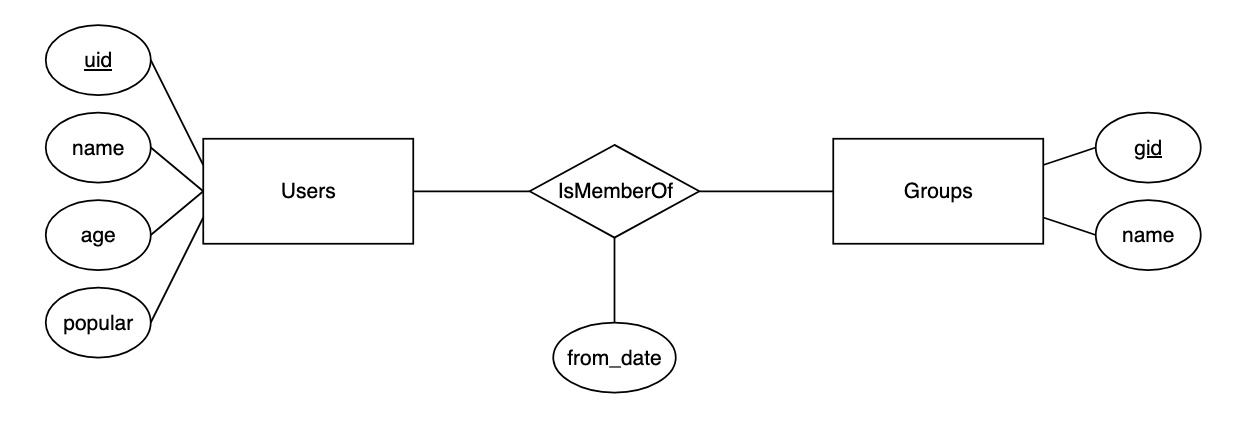
\includegraphics[scale=0.2]{img/social_media.png}
        \caption{Social media database ER diagram.} 
        \label{fig:social_media}
      \end{figure}

      Note that the \textit{from} attribute must be a part of the Member relation since it isn't uniquely associated with a user (a user can join multiple groups on different dates) or a group (two users can join a group on different dates). 
    \end{example}

    Therefore, we can associate an entity set and a relationship as relations. A minor detail is that relationships aren't really relations since the tuples in relations connect two entities, rather than the keys themselves, so some care must be taken to convert the entities into a set of attributes. 

    Therefore, we must determine if a relation models an entity or a relationship. There could also be multiple relationship sets between the same entity sets, e.g. if \textit{Member} and \textit{Likes} associates between \textit{Users} and \textit{Groups}. However, within a relationship set, there is an important set. 

    \begin{theorem}
      In a relationship set, each relationship is uniquely identified by the entities it connects. 
    \end{theorem}

    If there is an instance that someone joins, leaves, and rejoins a group, then we can modify our design by either: 
    \begin{enumerate}
      \item overwritting the first date joined 
      \item making another relation \textit{MembershipRecords} which has a date also part of the key, which will capture historical membership.  
    \end{enumerate}

    \subsubsection{Multiplicity of Binary Relationships}

      \begin{definition}[Multiplicity of Relationships]
        Given that $E$ and $F$ are entity sets, 
        \begin{enumerate}
          \item \textit{Many-many}: Each entity in E is related to $0$ or more entities in $F$ and vice versa. There are no restrictions, and we have \textit{IsMemberOf(\underline{uid}, \underline{gid})}. 

          \begin{figure}[H]
            \centering 
            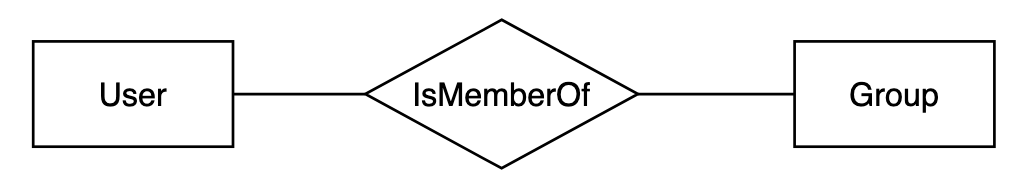
\includegraphics[scale=0.3]{img/ismember.png}
            \caption{} 
            \label{fig:ismember}
          \end{figure}


          \item \textit{Many-One}: Each entity in $E$ is related to $0$ or $1$ entity in $F$, but each entity in $F$ is related to $0$ or more in $E$. If $E$ points to $F$, then you can just think that this is an injective function, and we have \textit{IsOwnedBy(\underline{gid}, uid)}. If we have a rounded arrow, this means that for each group, its owner \textit{must} exist in \textit{Users} (so no $0$). 

          \begin{figure}[H]
            \centering 
            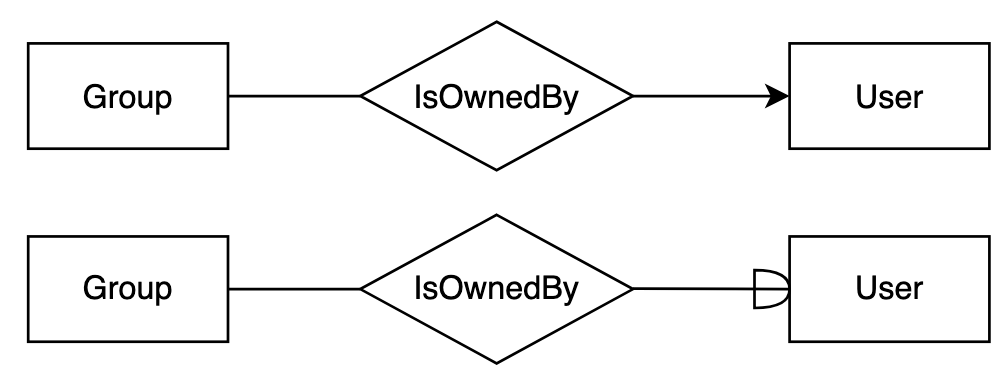
\includegraphics[scale=0.3]{img/isowned.png}
            \caption{} 
            \label{fig:isowned}
          \end{figure}


        \item \textit{One-One}: Each entity in $E$ is related to $0$ or $1$ entity in $F$ and vice versa. We can have either \textit{IsLinkedTo(\underline{uid}, twitter\_uid)} or \textit{IsLinkedTo(uid, \textit{twitter\_uid})} and must choose a primary key from these two possible keys.  

        \begin{figure}[H]
          \centering 
          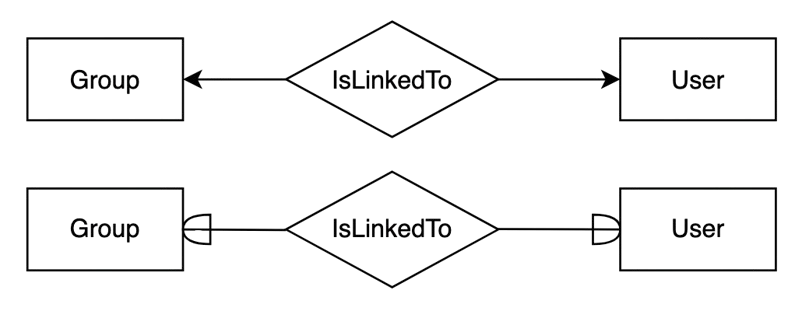
\includegraphics[scale=0.3]{img/islinked.png}
          \caption{} 
          \label{fig:islinked}
        \end{figure}

        \end{enumerate}
      \end{definition}


      You may notice that multiplicity and functional dependence are very similar that is. If we have two relations $R, S$ and have a relationship pointing from $R$ to $S$, then this states the FD $\mathbf{r} \mapsto \mathbf{s}$! Say that the keys are $\mathbf{k}_R, \mathbf{k}_S$, respectively. Then, we have 
      \begin{equation}
        \mathbf{k}_R \mapsto \mathbf{r} \mapsto \mathbf{s} \mapsto \mathbf{k}_S
      \end{equation} 

      \begin{example}[Movie Stars]
        Given the relations 
        \begin{enumerate}
          \item \textit{Movies(\underline{title, year}, length, name)}
          \item \textit{Stars(\underline{name}, address)} of a movie star and their address. 
          \item \textit{Studios(\underline{name}, address)} 
          \item \textit{StarsIn(\underline{star\_name}, \underline{movie\_name}, \underline{movie\_year})} 
          \item \textit{Owns(studio\_name, \underline{movie\_name}, \underline{movie\_year})}
        \end{enumerate}
        We have the following ER diagram 
        \begin{figure}[H]
          \centering 
          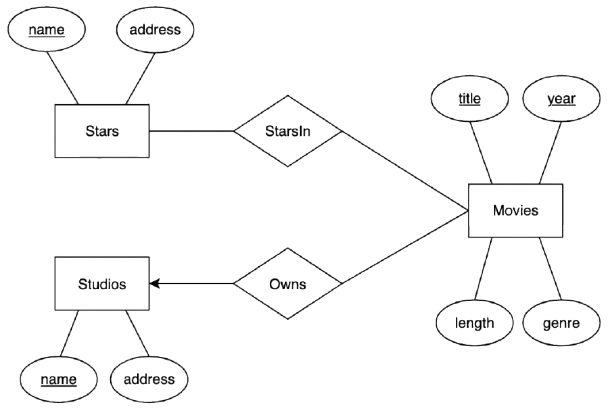
\includegraphics[scale=0.3]{img/movie_stars.png}
          \caption{Movie stars. } 
          \label{fig:movie_stars}
        \end{figure}
      \end{example}

      \begin{example}[Relationship within Itself]
        Sometimes, there is a relationship of an entity set with itself. This gives the relations 
        \begin{enumerate}
          \item \textit{Users(\underline{uid}, ...)} 
          \item \textit{IsFriendOf(\underline{uid1}, \underline{uid2})} 
          \item \textit{IsChildOf(\underline{child\_uid}, parent\_uid)}
        \end{enumerate}
        This can be modeled by the following. Note that 
        \begin{enumerate}
          \item users have no limitations on who is their friend. 
          \item assuming that all parents are single, a person can have at most one parent, so we have an arrow.  
        \end{enumerate}
        \begin{figure}[H]
          \centering 
          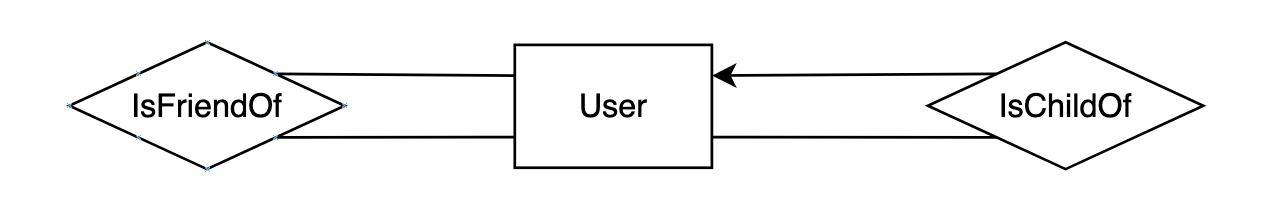
\includegraphics[scale=0.3]{img/within_itself.png}
          \caption{} 
          \label{fig:within_itself}
        \end{figure}
      \end{example}

    \subsubsection{Multiplicity of Multiway Relationships}

      Sometimes, it is necessary to have a relationship between 3 or more entity sets. It can be confusing to contruct the relations with the necessary keys. A general rule of thumb for constructing the relation of a relationship is 
      \begin{enumerate}
        \item Everything that the arrows point into are not keys.   
        \item Everything else are keys. So the arrow stumps are keys. 
      \end{enumerate}

      \begin{example}[Movie Stars]
        Suppose that we wanted to model \textit{Contract} relationship involving a studio, a star, and a movie. This relationships represents that a studio had contracted with a particular star to act in a particular movie. We want a contract to be owned by one studio, but one studio can have multiple contracts for different combinations of stars and movies. This gives the relations 
        \begin{enumerate}
          \item \textit{Stars(\underline{name}, address)} 
          \item \textit{Movies(\underline{title, year}, length, name)} 
          \item \textit{Studios(\underline{name}, address)} 
          \item \textit{Contracts(\underline{star\_name}, \underline{movie\_name}, studio\_name)}
        \end{enumerate}
        \begin{figure}[H]
          \centering 
          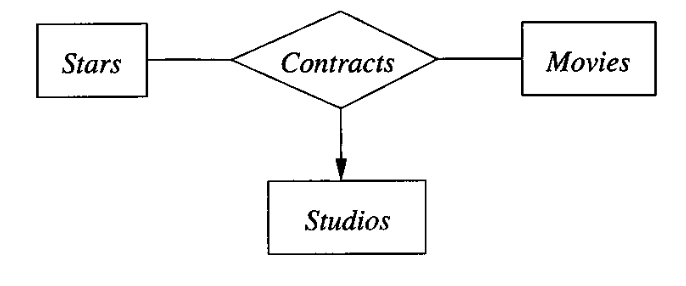
\includegraphics[scale=0.4]{img/contracts.png}
          \caption{} 
          \label{fig:contracts}
        \end{figure}
        We can make this even more complex by modifying contracts to have a studio of the star and the producing studio. 
        \begin{enumerate}
          \item \textit{Contracts(\underline{star\_name}, \underline{movie\_name}, produce\_studio\_name, star\_studio\_name)}
        \end{enumerate}
        \begin{figure}[H]
          \centering 
          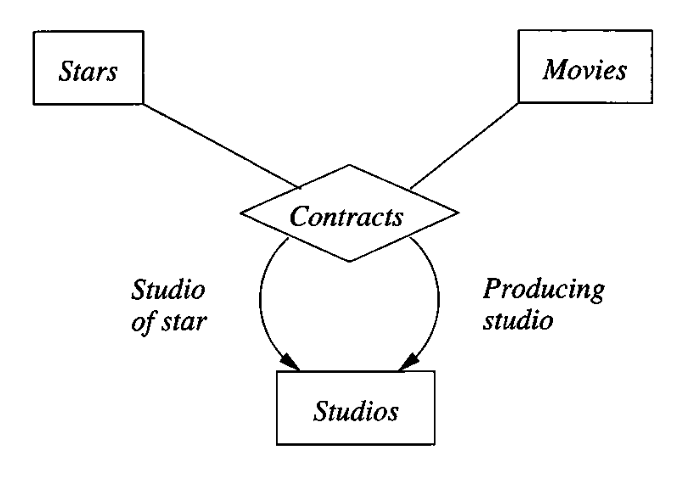
\includegraphics[scale=0.4]{img/four_ary.png}
          \caption{} 
          \label{fig:four_ary}
        \end{figure}
        Note that contracts can also have attributes, e.g. salary or time period. 
      \end{example}

      \begin{example}[Social Media]
        In a 3-ary relationship a user must have an initiator in order to join a group. In here, the \textit{isMemberOf} relation has an initiator, which must be unique for each initiated member, for a given group. 
        \begin{enumerate}
          \item \textit{User(\underline{uid}, ...)} 
          \item \textit{Group(\underline{gid}, ...)} 
          \item \textit{IsMemberOf(\underline{member}, initiator, \underline{gid})} since a member must have a unique pair of initiator/group that they are in. 
        \end{enumerate}
        \begin{figure}[H]
          \centering 
          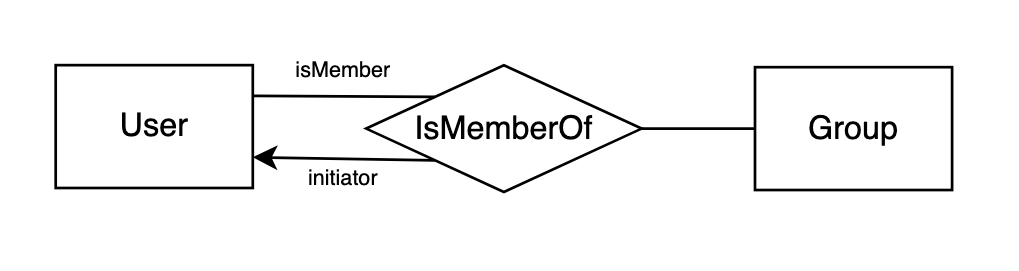
\includegraphics[scale=0.3]{img/three_ary.png}
          \caption{} 
          \label{fig:three_ary}
        \end{figure}
      \end{example}

      But can we model n-ary relationships with only binary relationships? Our intuition says we can't, for the same reasons that we get lossy decomposition into 2-attribute schemas when we try to satisfy BCNF. 
      \begin{figure}[H]
        \centering 
        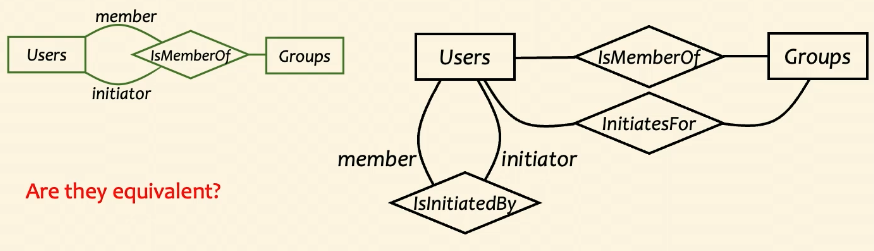
\includegraphics[scale=0.4]{img/nary_vs_binary.png}
        \caption{Attempt at reducing nary to binary ER relationships. } 
        \label{fig:}
      \end{figure}
      \begin{enumerate}
        \item u1 is in both g1 and g2, so \textit{IsMemberOf} contains both (u1, g1) and (u2, g2)
        \item u2 served as both an initiator in both g1 and g2, so \textit{InitiatesFor} contains both (g1, u2) and (g2, u2). 
        \item But in reality, u1 was initiated by u2 for g1 but not u2 for g2. This contradicts the information that you would get when joining the \textit{IsMemberOf} and \textit{InitiatesFor} relations. 
      \end{enumerate}
      Therefore, combining binary relations may generate something spurious that isn't included in the n-ary relationship. 

    \subsubsection{Subclasses of Entity Sets}

      Sometimes, an entity set contains certain entities that have special properties not associated with all members of the set. We model this by using a \textbf{isa} relationship with a triangle. 
      
      \begin{figure}[H]
        \centering 
        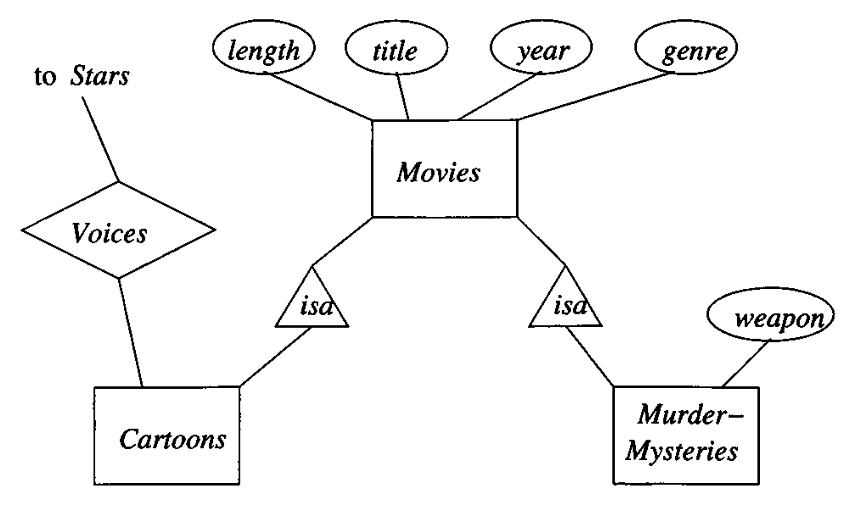
\includegraphics[scale=0.4]{img/isa.png}
        \caption{There are two types of movies: cartoons and murder-mysteries, which can have their own sub-attributes and their own relationships.} 
        \label{fig:isa}
      \end{figure}

      Suppose we have a tree of entity sets, connected by \textit{isa} relationships. A single entity consists of \textit{components} from one or more of these entity sets, and each component is inherited from its parent. 

  \subsection{Design Principles} 

    The first thing we should consider is the multiplicity, which is really context dependent. The second thing is redundancy, which we have mentioned through anomalies before.  

  \subsection{Weak Entity Sets}

    It is possible for an entity set's key to be composed of attributes, some or all of which belong to another entity set. There are two reasons why we need weak entity sets. 
    \begin{enumerate}
      \item Sometimes, entity sets fall into a hierarchy based on classifications unrelated to the \textit{isa} hierarchy. If entities of set $R$ are subunits of entities in set $F$, it is possible that the names of $R$-entities are not unique until we take into account the name of its $S$-entity.\footnote{Think of university rooms in different buildings.}
      \item The second reason is that we want to eliminate multiway relationships, which are not common in practice anyways. These weak entity sets have no attributes and have keys purely from its supporting sets. 
    \end{enumerate}

    \begin{definition}[Weak Entity Set]
      A \textbf{weak entity set} $R$ (double rectangles) depends on other sets. It is an entity set that 
      \begin{enumerate}
        \item has a key consisting of 0 or more of its own attributes, and 
        \item has key attributes from \textbf{supporting entity sets} that are reached by many-one \textbf{supporting relationships} (double diamonds) from it to other sets $S$. 
      \end{enumerate}
      It must satisfy the following. 
      \begin{enumerate}
        \item The relationship $T$ must be binary and many-one from $R$ to $S$. 
        \item $T$ must have referential integrity from $R$ to $S$ (since these are keys and therefore must exist in supporting sets), which is why we have a rounded arrow. 
        \item The attributes that $S$ supplies for the key of $R$ must be key attributes of $S$, unless $S$ is also weak, and it will get keys from its supporting entity set. 
        \item If there are several different supporting relationships from $R$ to the same $S$, then each relationship is used to supply a copy of the key attributes of $S$ to help form the key of $R$. 
      \end{enumerate}
      If an entity set supplies any attributes for its own key, then those attributes will be underlined. 
    \end{definition}

    \begin{example}
      To specify a location, it is not enough to specify just the seat number. The room number, and the building name must be also specified to provide the exact location. There are no extra attributes needed for this subclass, which is why a \textit{isa} relationship doesn't fit into this. 
      \begin{figure}[H]
        \centering 
        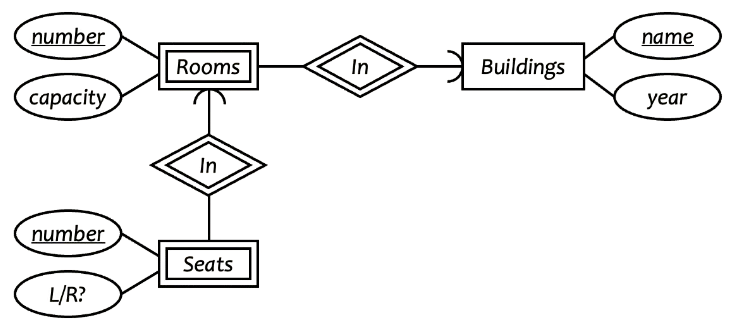
\includegraphics[scale=0.4]{img/weak_entity.png}
        \caption{Specifying a seat is not enough to determine the exact location in a university. We must know the room number and the building to fully identify it. Note that we must keep linking until we get to a regular, non-weak entity. } 
        \label{fig:weak_entity}
      \end{figure}
    \end{example}

    We generally want to use a weak entity set if an entity does not have attributes to define itself. 
    
    \begin{example}
      Say that we want to make a database with the constraints. 
      \begin{enumerate}
        \item For states, record the name and capital city. 
        \item For counties, record the name, area, and location (state) 
        \item For cities, record the name, population, and location (county and state) 
        \item Names of states should be unique. 
        \item Names of counties are unique within a state. 
        \item Names of cities are unique within a county. 
        \item A city is always located in a single county. 
        \item A county is always located in a single state. 
      \end{enumerate}
      Then, our ER diagram may look like 
      \begin{figure}[H]
        \centering 
        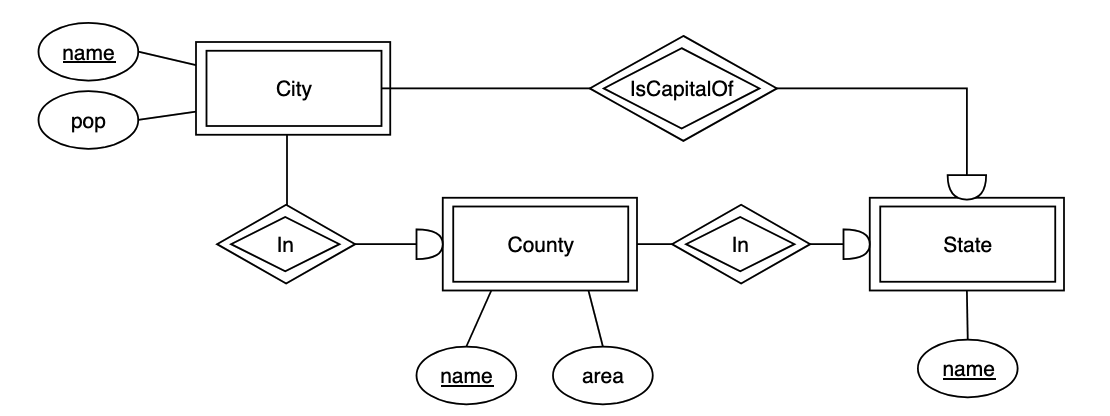
\includegraphics[scale=0.3]{img/city1.png}
        \caption{A weakness is that this doesn't prevent a city in state $X$ from being the capital of another state $Y$.} 
        \label{fig:city1}
      \end{figure}
    \end{example}

    \begin{example}
      Design a database with the following. 
      \begin{enumerate}
        \item A station has a unique name and address, and is either an express station or a local station. 
        \item A train has a unique number and engineer, and is either an express or local train. 
        \item A local train can stop at any station. 
        \item An express train only stops at express stations. 
        \item A train can stop at a station for any number of times during a train. 
        \item Train schedules are the same every day. 
      \end{enumerate}
      Then, our ER diagram may look like 
      \begin{figure}[H]
        \centering 
        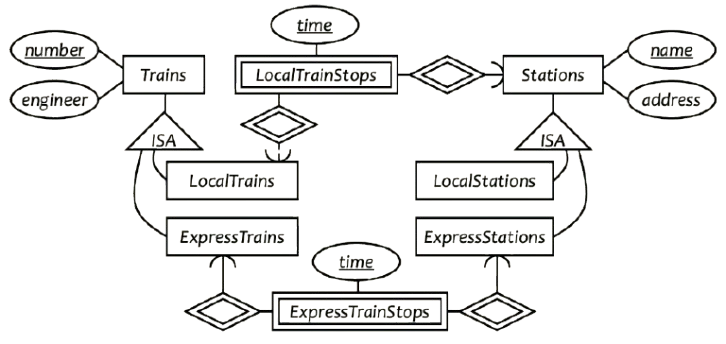
\includegraphics[scale=0.4]{img/train1.png}
        \caption{} 
        \label{fig:train1}
      \end{figure}
      
    \end{example}

  \subsection{Translating ER Diagrams to Relational Designs}

    One a simple level, converting an ER diagram to a relational database schema is straightforward. Here are some rules we list. 

    \begin{theorem}[Converting Entity Sets]
      Turn each entity set into a relation with the same set of attributes. 
    \end{theorem}

    \begin{theorem}[Converting Relationships]
      Replace a relationship by a relation whose attributes are the keys for the connected entity sets along with its own attributes. If an entity set is involved several times in a relationship, then its key attributes are repeated, so you must rename them to avoid duplication.
    \end{theorem}

    \begin{theorem}[Reduce Repetition for Many-One Relationships]
      We can actually reduce repetition for many-one relationships. For example, if there is a many-one relationship $T$ from relation $R$ to relation $S$, then $\mathbf{r}$ functionally determines $\mathbf{s}$, so we can combine them into one relation consisting of 
      \begin{enumerate}
        \item all attributes of $R$. 
        \item key attributes of $S$. 
        \item Any attributes belonging to relationship $T$. 
      \end{enumerate}
    \end{theorem}
    
    \begin{theorem}[Handling Weak Entity Sets]
      To build weak entity sets, we must do three things. 
      \begin{enumerate}
        \item The relation for weak entity set $W$ must include its own attributes, all key (but not non-key) attributes of supporting entity sets, and all attributes for supporting relationships for $W$. 
        \item The relation for any relationship where $W$ appears must use the entire set of keys gotten from $W$ and its supporting entity sets. 
        \item Supporting relationships should not be converted since they are many-one, so we can use the reduce repetition for many-one relationships rule above. 
      \end{enumerate}
    \end{theorem}

    \begin{example}
      To translate the seat, rooms, and buildings diagram, 
      \begin{figure}[H]
        \centering 
        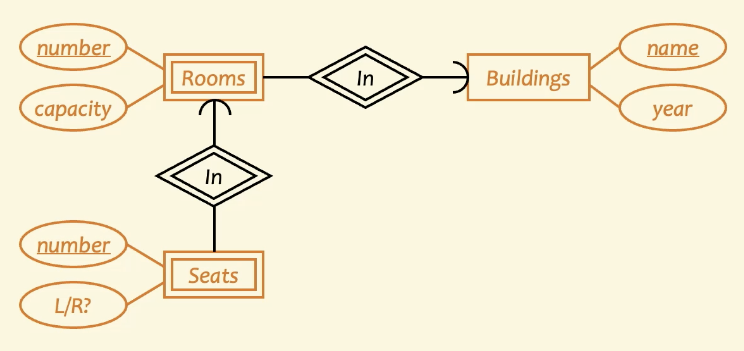
\includegraphics[scale=0.4]{img/seat.png}
        \caption{} 
        \label{fig:seat}
      \end{figure}
      we have 
      \begin{enumerate}
        \item \textit{Building(\underline{name}, year)} 
        \item \textit{Room(\underline{building\_name}, \underline{room\_num}, capacity)}
        \item \textit{Seat(\underline{building\_name}, \underline{room\_num}, \underline{seat\_num}, left\_or\_right)}
      \end{enumerate}
      Note that we do not need to convert the relationships since they are contained within the entity set relations. So ignore double diamonds. 
    \end{example}

    \begin{figure}[H]
      \centering 
      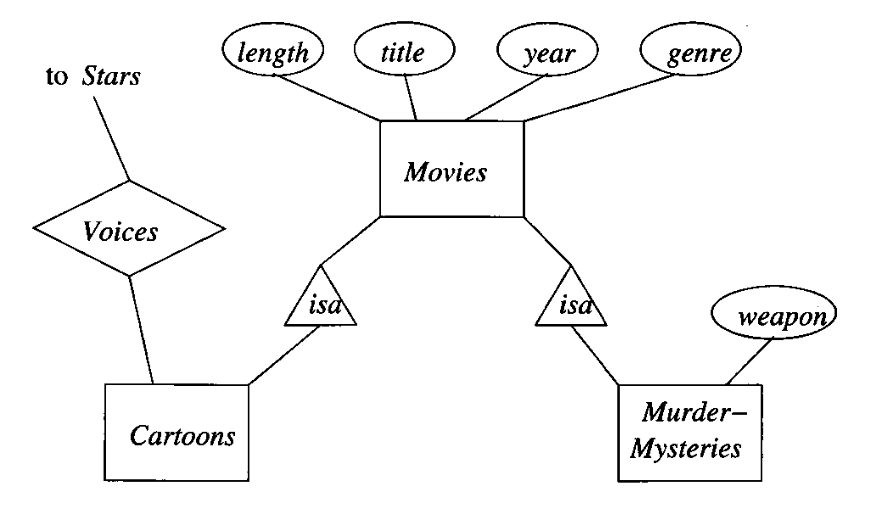
\includegraphics[scale=0.3]{img/movie_hierarchy.png}
      \caption{A figure of the movie hierarchy for convenience. } 
      \label{fig:movie_hierarchy}
    \end{figure}

    \begin{theorem}[Converting Subclass Structures]
      To convert subclass structure with a \textit{isa} hierarchy, there are multiple ways we can convert them. 
      \begin{enumerate}
        \item \textit{E/R Standard}. An entity is in all superclasses and only contains the attributes its own subclass. For each entity set $R$ in the hierarchy, create a relation that includes the key attributes from the root and any attributes belonging to $R$. This gives us 
          \begin{enumerate}
            \item \textit{Movies(title, year, length, genre)}
            \item \textit{MurderMysteries(title, year, weapon)}
            \item \textit{Cartoons(title, year)}
          \end{enumerate}
        \item \textit{Object Oriented}. For each possible subtree that includes the root, create one relation whose schema includes all the attributes of all entity sets in the subtree.
          \begin{enumerate}
            \item \textit{Movies(title, year, length, genre)} 
            \item \textit{MoviesC(title, year, length, genre)} 
            \item \textit{MoviesMM(title, year, length, genre, weapon)}
            \item \textit{MoviesCMM(title, year, length, genre, weapon)}
          \end{enumerate}
          Additionally, the relationship would be \textit{Voices(title, year, starName)}. 
        \item \textit{Null Values}. Create one relation for the entire hierarchy containing all attributes of all entity sets. Each entity is one tuple, and the tuple has null values for attributes the entity does not have. We would in here always have a single schema. 
          \begin{enumerate}
            \item \textit{Movie(title, year, length, genre, weapon)}
          \end{enumerate}
      \end{enumerate}
    \end{theorem}

    Note that the difference between the first two is that in ER, \textit{MurderMysteries} does not contain the attributes of its superclass, while in OO, it does. 

    As you probably notice, each standard has pros and cons. The nulls approach uses only one relation, which is simple and nice. To filter out over all movies, E/R is nice since we only filter through \textit{Movies}, whilst in OO we have to go through all relations. However, when we want to filter movies that are both Cartoons and Murder Mysteries, then OO is better since we can only select from \textit{MoviesCMM} rather than having to go through multiple relations for ER or filter out with further selections in Null. Also, OO uses the least memory, since it doesn't waste space on null values on attributes.  


    \begin{example}
      Let's put this all together to revisit the train station example. 
      \begin{figure}[H]
        \centering 
        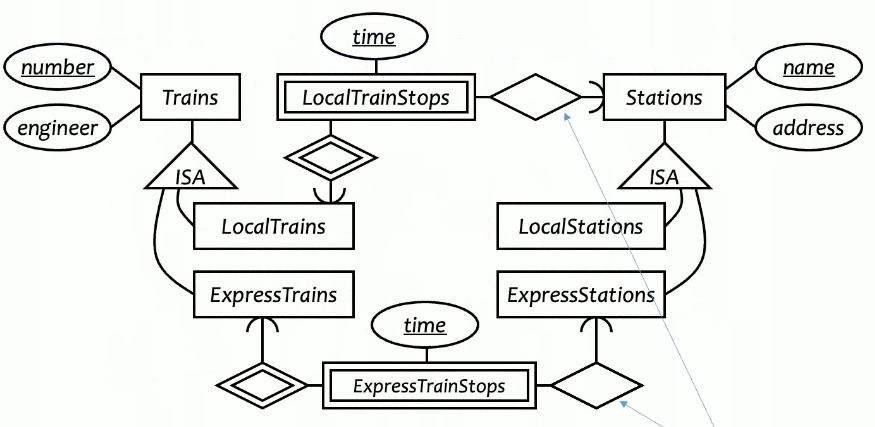
\includegraphics[scale=0.4]{img/final_station.png}
        \caption{For convenience} 
        \label{fig:final_station}
      \end{figure}
      We can use the ER standard to define the first 6 regular relations in single rectangles.  
      \begin{enumerate}
        \item \textit{Train(\underline{number}, engineer)}
        \item \textit{LocalTrain(\underline{number}}
        \item \textit{ExpressTrain(\underline{number}}
        \item \textit{Station(\underline{name}, address)}
        \item \textit{LocalStation(\underline{name})}
        \item \textit{ExpressStation(\underline{name})}
      \end{enumerate}
      Then we can construct the weak entity sets. 
      \begin{enumerate}
        \item \textit{LocalTrainStops(\underline{local\_train\_num}, \underline{time})}
        \item \textit{ExpressTrainStops(\underline{express\_train\_num}, \underline{time})}
      \end{enumerate}
      Then we can construct the relationships (marked with the arrows).  
      \begin{enumerate}
        \item \textit{LocalTrainStopsAtStation(\underline{local\_train\_number}, \underline{time}, station\_name)}
        \item \textit{ExpressTrainStopsAtStation(\underline{express\_train\_number}, \underline{time}, express\_station\_name)}
      \end{enumerate}
      Note that we can simplify these 10 relations to 8. For example, the \textit{LocalTrain} and \textit{LocalStation} relations are redundant since it can be computed as 
      \begin{align}
        LocalTrain & = \pi_{number} (Train) - ExpressTrain \\
        LocalStation & = \pi_{number} (Station) - ExpressStation
      \end{align}
      There is a tradeoff since it's an extra computation when checking. However, if we had used the Null Value strategy, this would be a lot simpler, and we can use value constraints on the train and station type, which can be implemented in the DBMS (though not directly in the ER diagram). 
    \end{example}

\section{Intermediate SQL} 

    We have went over the basic SQL queries that were directly translations of relational algebra. 

  \subsection{Bags}

    We were used to working with sets, which don't allow duplicate elements, but let's talk about \textit{multisets}, or \textbf{bags}, which do. Why is this advantageous? 
    \begin{enumerate}
      \item To take the union of two bags, we can just add everything into the other without going through to check for duplicates. 
      \item When we project relations as bags, we also don't need to search through all pairs to find duplicates. 
    \end{enumerate}
    This allows for efficiency at the cost of memory. 

    Recall that the \texttt{UNION}, \texttt{EXCEPT}, and \texttt{INTERSECT} are set semantics that removes duplicates in the input tables first and then removes duplicates in the result. 

    \begin{definition}[Bag Operations]
      However, we can also use bag semantics. We can think of each row $a$ having an implicit count of times $c_a$ it appears in the table.  
      \begin{enumerate}
        \item \textbf{Bag union} sums up the counts from two tables. 
        \item \textbf{Bag difference} does a proper-subtract\footnote{Subtracts the counts and truncates counts to $0$ if negative. So $\{a, a\} - \{a, a, a\} = \{\}$.} 
        \item \textbf{Bag intersection} takes the minimum of the two counts. 
      \end{enumerate}
      This is analogous to the \texttt{UNION ALL}, \texttt{EXCEPT ALL}, and \texttt{INTERSECT ALL} operations in SQL. Given that 
      \begin{enumerate}
        \item $\mathrm{Bag1} = \{1, 1, 2\}$
        \item $\mathrm{Bag2} = \{1, 2, 2\}$
      \end{enumerate}
      We have 
      \begin{lstlisting}
        (SELECT * FROM Bag1) 
        UNION ALL 
        (SELECT * FROM Bag2);     // {1, 1, 1, 2, 2, 2}

        (SELECT * FROM Bag1) 
        EXCEPT ALL 
        (SELECT * FROM Bag2);     // {1}

        (SELECT * FROM Bag1) 
        INTERSECT ALL 
        (SELECT * FROM Bag2);     // {1, 2}
      \end{lstlisting}
    \end{definition}

    \begin{example}
      Look at these two operations on the schema \texttt{Poke(uid1, uid2, timestamp)}. 

      \noindent\begin{minipage}{.5\textwidth}
      \begin{lstlisting}[]{Code}
        (SELECT uid1 FROM Poke) 
        EXCEPT 
        (SELECT uid2 FROM Poke); 
      \end{lstlisting}
      \end{minipage}
      \hfill
      \begin{minipage}{.49\textwidth}
      \begin{lstlisting}[]{Output}
        (SELECT uid1 FROM Poke) 
        EXCEPT ALL
        (SELECT uid2 FROM Poke); 
      \end{lstlisting}
      \end{minipage}
      The first operation returns all users who poked others but were never poked, while the second returns all users who poked others more than they were poked. 
    \end{example}

  \subsection{Nested Queries and Subqueries} 

    We have so far worked with a single query consisiting of a single select statement. However, we can extend this. 

    \begin{definition}[\texttt{EXISTS}]
      The \texttt{EXISTS}(subquery) keyword checks if a subquery is empty or not, and \texttt{NOT EXISTS} checks the negation. 
    \end{definition}

    \begin{example}[Ages]
      Given \textit{User(name, age)}, say that we want to get all users whose age is equal to a person named Bart. Then, we want to select all users from the relation. For each user, we perform the subquery where this original tuple age coincides the others age and the others name is Bart. The outer query only returns those rows for which the \texttt{EXISTS} subquery returned true. Then we can write the two equivalent queries. 

      \noindent\begin{minipage}{.5\textwidth}
      \begin{lstlisting}[]{Code}
        SELECT * 
        FROM User as u
        WHERE EXISTS(SELECT * FROM User
                      WHERE name = "Bart" 
                      AND age = u.age); 
      \end{lstlisting}
      \end{minipage}
      \hfill
      \begin{minipage}{.49\textwidth}
      \begin{lstlisting}[]{Output}
        SELECT * 
        FROM User 
        WHERE age IN(SELECT age 
                      FROM User 
                      WHERE name = 'Bart'); 
      \end{lstlisting}
      \end{minipage}

      The left is a \textbf{correlated subquery}, which is a query that needs a parameter from the main query and are generally slower. To understand this, you should always look in the following order. 
      \begin{enumerate}
        \item \texttt{FROM}. Look at where we are querying from. 
        \item \texttt{WHERE}. Find out if this condition is satisfied. 
        \item \texttt{SELECT}. Return all tuples that satisfies this condition. 
      \end{enumerate}
      However, this is not actually how the database system will do this. It will do it in an equivalent but more efficient way. 
    \end{example}

    Here is a very useful keyword that simplifies complex nested queries, one example of a \textbf{common table expression (CTEs)}. 
    
    \begin{definition}[\texttt{WITH}]
      The \texttt{WITH} clause aliases many relations returned from queries. 
      \begin{lstlisting}
        WITH Temp1 AS (SELECT ...), 
             Temp2 AS (SELECT ...) 
        SELECT X, Y 
        FROM Temp1, Temp2 
        WHERE ...
      \end{lstlisting}
    \end{definition}

    \begin{example}
      To extend the Bart age example, we can think of temporarily storing a query of only Bart's ages, and then comparing it when doing the main query over \textit{User}. 
      \begin{lstlisting}
        WITH BartAge AS 
          (SELECT age 
          FROM User 
          WHERE name = 'Bart') 
        SELECT U.uid, U.name, U.pop, 
        FROM User U, BartAge B 
        WHERE U.age = B.age; 
      \end{lstlisting}
    \end{example}

  \subsection{Aggregate Functions} 

    \begin{definition}[Standard SQL Aggregate Functions]
      The aggregate functions offered are 
      \begin{enumerate}
        \item \texttt{COUNT} counts the number of rows in a query. \texttt{COUNT(DISTINCT att)} counts the distinct count of an attribute in a query. 
        \item \texttt{SUM} counts the sum of the values of an attribute in a query. 
        \item \texttt{AVG} is the average. 
        \item \texttt{MIN} is the minimum of an attribute. 
        \item \texttt{MAX} is the maximum of an attribute. 
      \end{enumerate}
    \end{definition}

    \begin{example}
      If we want to find the number of users under 18 and their average popularity, then we can write 
      \begin{lstlisting}
        SELECT COUNT(*), AVG(pop) 
        FROM User 
        WHERE age < 18; 
      \end{lstlisting}
    \end{example}

  \subsection{Group By} 

    \begin{definition}[\texttt{GROUP BY}]
      \texttt{GROUP BY att} is used when you want to group the query by equal values of the attributes. The syntax is 
      \begin{lstlisting}
        SELECT ... FROM ... WHERE ... 
        GROUP BY age; 
      \end{lstlisting}
      To parse this, first form the groups based on the same values of all attributes in the group by clause. Then, output only one row in the select clause per group. We can look at the following order
      \begin{enumerate}
        \item \texttt{FROM}. Look at where we are querying from. 
        \item \texttt{WHERE}. Find out if this condition is satisfied to filter the main query. 
        \item \texttt{GROUP BY}. Group rows according to the values of the GROUP BY columns. 
        \item \texttt{SELECT}. Compute the select query for each group. The number of groups should be equal to the number of rows in the final output. 
      \end{enumerate}
      Note that if a query uses aggregation/group by, every column referenced in select must be either aggregated or a group by column. 
    \end{definition}

    \begin{example}
      If we want to find the number of users in a certain age and their average popularity, for all ages, then we can write 
      \begin{lstlisting}
        SELECT age, AVG(pop) 
        FROM Usere
        GROUP BY age; 
      \end{lstlisting}
      You don't necessarily have to report the group by attribute in the select. The two following examples are perfectly fine, though in the right query, \texttt{age} may not functionally determine \texttt{AVG(pop)}. 

      \noindent\begin{minipage}{.5\textwidth}
      \begin{lstlisting}[]{Code}
        SELECT AVG(pop) 
        FROM User
        GROUP BY age; 
        
      \end{lstlisting}
      \end{minipage}
      \hfill
      \begin{minipage}{.49\textwidth}
      \begin{lstlisting}[]{Output}
        SELECT age, AVG(pop)  
        FROM User 
        GROUP BY age, name; 
      \end{lstlisting}
      \end{minipage}

      However, this left query is not syntactically correct since \texttt{name} is not in the group by clause or aggregated. This is true even if \texttt{age} functionally determines \texttt{name}. Neither is the right since the lack of a group by clause means that the aggregate query is over the entire relation, which has multiple uid values. 

      \noindent\begin{minipage}{.5\textwidth}
      \begin{lstlisting}[]{Code}
        SELECT age, name, AVG(pop) 
        FROM User
        GROUP BY age; 
      \end{lstlisting}
      \end{minipage}
      \hfill
      \begin{minipage}{.49\textwidth}
      \begin{lstlisting}[]{Output}
        SELECT uid, MAX(pop) 
        FROM User; 
        .
      \end{lstlisting}
      \end{minipage}
    \end{example}

    As you can see, this is great to use for aggregate functions. If there is no group by clause, this is equivalent to grouping everything together.  

    \begin{example}
      Given the relation 

      \begin{table}[H]
        \centering
        \begin{tabular}{|c|c|c|}
          \hline
          \textbf{A} & \textbf{B} & \textbf{C} \\
          \hline
          1 & 1 & 10 \\ 
          2 & 1 & 8 \\ 
          1 & 1 & 10 \\ 
          2 & 3 & 8 \\ 
          2 & 1 & 6 \\ 
          2 & 2 & 2 \\ 
          \hline
        \end{tabular}
        \caption{Original relation. }
        \label{tab:groupby}
      \end{table}
    
      Running the query 
      \begin{lstlisting}
        SELECT A, B, SUM(C) AS S 
        FROM R 
        GROUP BY A, B; 
      \end{lstlisting}
      gives 
      
      \begin{table}[H]
        \centering
        \begin{tabular}{|c|c|c|}
          \hline
          \textbf{A} & \textbf{B} & \textbf{S} \\
          \hline
          1 & 1 & 20 \\ 
          2 & 1 & 14 \\ 
          2 & 3 & 8 \\ 
          2 & 2 & 2 \\ 
          \hline
        \end{tabular}
        \caption{Our query. }
        \label{tab:groupby_output}
      \end{table}
    \end{example}

  \subsection{Having} 

    \begin{definition}[\texttt{HAVING}]
      If you want to filter out groups having certain conditions, you must use the \texttt{HAVING} keyword rather than \texttt{WHERE}. The syntax is 
      \begin{lstlisting}
        SELECT A, B, SUM(C) FROM ... WHERE ... 
        GROUP BY ... 
        HAVING SUM(C) < 10; 
      \end{lstlisting}
      You should look at the \texttt{HAVING} clause after you look at the \texttt{GROUP BY} but before \texttt{SELECT}. 
    \end{definition}

    \begin{example}
      Given the relation 

      \begin{table}[H]
        \centering
        \begin{tabular}{|c|c|c|}
          \hline
          \textbf{A} & \textbf{B} & \textbf{C} \\
          \hline
          1 & 1 & 10 \\ 
          2 & 1 & 8 \\ 
          1 & 1 & 10 \\ 
          2 & 3 & 8 \\ 
          2 & 1 & 6 \\ 
          2 & 2 & 2 \\ 
          \hline
        \end{tabular}
        \caption{Original relation. }
        \label{tab:groupby2}
      \end{table}
    
      Running the query 
      \begin{lstlisting}
        SELECT A, B, SUM(C) AS S 
        FROM R 
        GROUP BY A, B 
        HAVING SUM(C) > 8; 
      \end{lstlisting}
      gives 
      
      \begin{table}[H]
        \centering
        \begin{tabular}{|c|c|c|}
          \hline
          \textbf{A} & \textbf{B} & \textbf{S} \\
          \hline
          1 & 1 & 20 \\ 
          2 & 1 & 14 \\ 
          \hline
        \end{tabular}
        \caption{Our query. }
        \label{tab:groupby2_output}
      \end{table}
    \end{example}

    \begin{example}
      Given the schema \texttt{Sailor(sid, name, age, rating)}, to find the age of the youngest sailor with age at least 18, for each rating with at least 2 sailors, we can run the query. 
      \begin{lstlisting}
        SELECT S.rating, MIN(S.age) AS minage 
        FROM Sailors S 
        WHERE S.age >= 18
        GROUPBY S.rating 
        HAVING COUNT(*) > 1; 
      \end{lstlisting}

      \begin{figure}[H]
        \centering 
        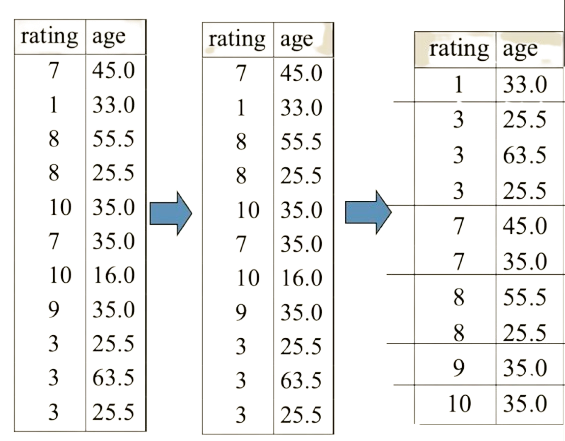
\includegraphics[scale=0.4]{img/sailors.png}
        \caption{The thought process.} 
        \label{fig:thought}
      \end{figure}
    \end{example}

    \begin{definition}[Scalar Subqueries]
      Sometimes, if a query returns 1 scalar, then you can use it in your \texttt{WHERE} clause. You must be sure that a query will return exactly 1 scalar (not $0$ and not more than $1$), or there will be a runtime error.  
    \end{definition}

    \begin{example}
      If we want to compute users with the same age as Bart, we can write 
      \begin{lstlisting}
        SELECT * FROM User 
        WHERE age = (SELECT age from User WHERE name = 'Bart'); 
      \end{lstlisting}
      However, we may not know if Bart functionally determines age, so we must be careful. 
    \end{example}

  \subsection{Quantified Subqueries}

    \begin{definition}[\texttt{ALL}, \texttt{ANY}]
      We have the following \textbf{quantified subqueries}, which performs a broadcasting condition and checks if all (\texttt{ALL}) or any (\texttt{ANY}) are true. 
    \end{definition}

    \begin{example}[Popular Users]
      Which users are the most popular? We can write this in two ways. 

      \noindent\begin{minipage}{.5\textwidth}
      \begin{lstlisting}[]{Code}
        SELECT * 
        FROM User 
        WHERE pop >= ALL(SELECT pop from User); 
        .
      \end{lstlisting}
      \end{minipage}
      \hfill
      \begin{minipage}{.49\textwidth}
      \begin{lstlisting}[]{Output}
        SELECT * 
        FROM User 
        WHERE NOT 
          (pop < ANY(SELECT pop from User)); 
      \end{lstlisting}
      \end{minipage}

      To review, here are more ways you can do the same query. 

      \noindent\begin{minipage}{.5\textwidth}
      \begin{lstlisting}[]{Code}
        SELECT * 
        FROM User AS u 
        WHERE NOT EXISTS  
          (SELECT * FROM User
          WHERE pop > u.pop); 
      \end{lstlisting}
      \end{minipage}
      \hfill
      \begin{minipage}{.49\textwidth}
      \begin{lstlisting}[]{Output}
        SELECT * FROM User 
        WHERE uid NOT IN 
          (SELECT u1.uid
          FROM User as u1, User as u2 
          WHERE u1.pop < u2.pop); 
      \end{lstlisting}
      \end{minipage}
    \end{example}

  \subsection{Incomplete Information}

    We are not guaranteed that we will have all data. What if there are some null values? We need some way to handle unknown or missing attribute values. 

    One way is to use a default value (like $-1$ for age), but this can mess with other operations, such as getting average values of certain groups of users, or can make computations harder since we have to first filter out users with \texttt{age=-1} before querying. 

    Another way is to use a valid bit for every attribute. For example, \textit{User(uid, name, age)} could map to \textit{User(uid, name, name\_valid, age, age\_valid)}, but this is not efficient as well. 

    A better solution is to decompose the table into multiple relations such that a missing value indicates a missing row in one of the subrelations. For example, we can decompose \texttt{User(uid, name, age, pop)} to 
    \begin{enumerate}
      \item \textit{UserID(uid)}
      \item \textit{UserName(uid, name)}
      \item \textit{UserAge(uid, age)}
      \item \textit{UserPop(uid, pop)}
    \end{enumerate}
    This is conceptually the cleanest solution but also complicates things. Firstly, the natural join wouldn't work, since compared to a single table with null values, the natural join of these tables would exclude all tuples that have at least one null value in them. 


    \begin{definition}[\texttt{NULL}]
      SQL's solution is to have a special value \texttt{NULL} indicating an unknown but not empty value. It has the following properties. 
      \begin{enumerate}
        \item It holds for every domain (null is the same for booleans, strings, ints, etc.). 
        \item Any operations like $+, -, \times, >$... leads to a \texttt{NULL} value. 
        \item All aggregate functions except \texttt{COUNT} return a \texttt{NULL}. \texttt{COUNT} also counts null values. 
      \end{enumerate}
    \end{definition}

    \begin{theorem}[Three-Valued Logic]
      Here is another way to implement the unknown logic with \textit{three-valued logic}. Suppose we set True=1, False=0. Then we can see that given statements $x, y$ which evaluate to $0, 1$, 
      \begin{enumerate}
        \item $x$ and $y$ is equivalent to $\min(x, y)$
        \item $x$ or $y$ is equivalent to $\max(x, y)$ 
        \item not $x$ is equivalent to $1 - x$
      \end{enumerate}
      It turns out that if we set unknown=0.5, then this logic also works out very nicely. Check it yourself. Therefore, \texttt{WHERE} and \texttt{HAVING} clauses only select rows for which the condition is True, not False or Unknown. 
    \end{theorem}

    \begin{example}[Warnings]
      Note that null breaks a lot of equivalences, leading to unintended consequences. 
      \begin{enumerate}
        \item The two are not equivalent since if we have nulls, the average ignores all nulls, while the second query will sum up all non-nulls and divide by the count including the nulls. 
        \begin{lstlisting}
          SELECT AVG(pop) FROM User; 
          SELECT SUM(pop) / COUNT(*) FROM User; 
        \end{lstlisting}

        \item The two are also not equivalent since \texttt{pop = pop} is not True, but Unknown, for nulls, so it would not return nulls. The first query would return all tuples, even nulls. 
        \begin{lstlisting}
          SELECT * from User; 
          SELECT * from User WHERE pop = pop; 
        \end{lstlisting}

        \item Never compare equality with null, since this never outputs True. Rather, you should use the special keywords \texttt{IS NULL} and \texttt{IS NOT NULL}. 
          \begin{lstlisting}
            SELECT * FROM User WHERE pop = NULL; // never returns anything 
            SELECT * FROM User WHERE pop IS NULL; // correct 
          \end{lstlisting}
      \end{enumerate}
    \end{example}


  \subsection{Joins} 
    
    Take a look at the following motivating example. Suppose we want to find all members and their respective groups from \textit{Group(gid, name)}, \textit{Member(uid, gid)}, \textit{User(uid, name)}. Then we can write the query 
    \begin{lstlisting}
      SELECT g.gid, g.name AS gname, 
          u.uid, u.name AS uname 
      FROM Group g, Member m, User u 
      WHERE g.gid = m.gid AND m.uid = u.uid; 
    \end{lstlisting}
    This looks fine, but what happens if \textit{Group} is empty? That is, there is a group in the \textit{Group} relation but does not appear in the \textit{Member} relation. Then, \texttt{m.gid} will evaluate to False and would not appear in the joined table, which is fine, but what if we wanted to make sure all groups appeared in this master membership table? If a group is empty, we may want it to just have null values for \texttt{uid} and \texttt{uname}. In this case, we want to use outer join. 

    \begin{definition}[Outer Joins]
      An outer join guarantees that we have all elements in one or more tables. 
      \begin{enumerate}
        \item \texttt{(INNER) JOIN}: Returns records that have matching values in both tables, with the notation $R \bowtie S$. 
        \item \texttt{LEFT (OUTER) JOIN}: Returns all records from the left table, and the matched records from the right table with potential NULLs, with notation $R \lojoin S$. 
        \item \texttt{RIGHT (OUTER) JOIN}: Returns all records from the right table, and the matched records from the left table with potential NULLs, with notation $R \rojoin S$. 
        \item \texttt{FULL (OUTER) JOIN}: Returns all records when there is a match in either left or right table with potential NULLs, with notation $R \fojoin S$. 
      \end{enumerate}

      \begin{figure}[H]
        \centering 
        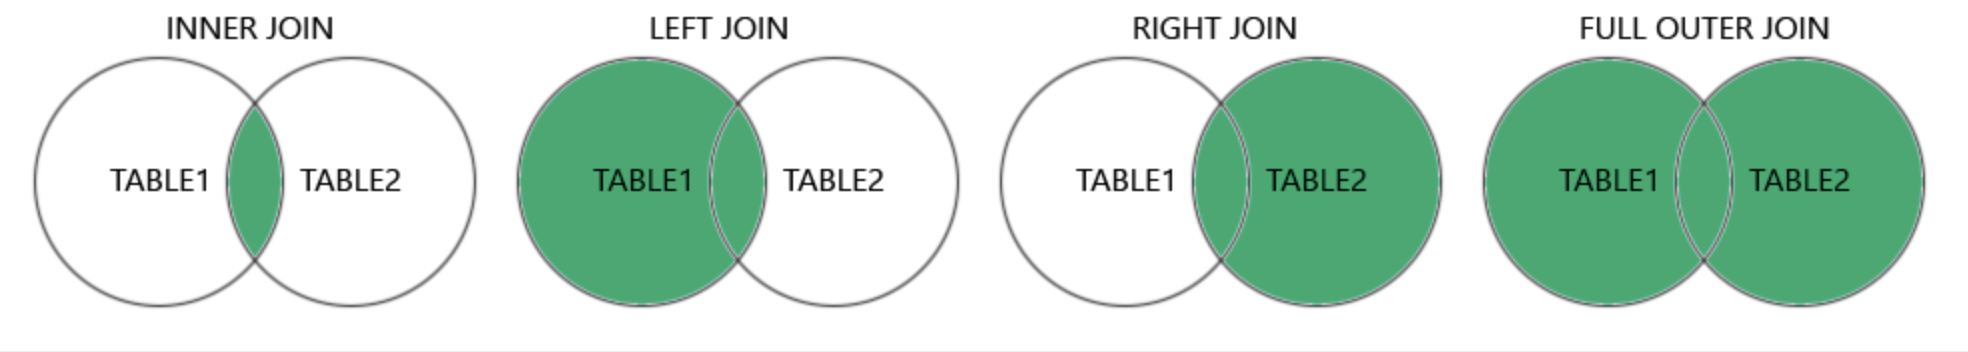
\includegraphics[scale=0.4]{img/outerjoin.png}
        \caption{Nice diagram from W3Schools.} 
        \label{fig:outerjoin}
      \end{figure}

      The SQL syntax is below. 
      \begin{lstlisting}
        // inner joins, you can use ON rather than WHERE
        SELECT * FROM Group JOIN Member
          ON Group.gid = Member.gid; 

        SELECT * FROM Group LEFT OUTER JOIN Member
          ON Group.gid = Member.gid; 

        SELECT * FROM Group RIGHT OUTER JOIN Member
          ON Group.gid = Member.gid; 

        SELECT * FROM Group RIGHT OUTER JOIN Member
          ON Group.gid = Member.gid; 
      \end{lstlisting}
    \end{definition}

    \begin{example}[Complex Example with Beers]
      Given the schemas 
      \begin{enumerate}
        \item \textit{Frequents(drinker, bar, times\_a\_week)}, 
        \item \textit{Serves(bar, beer, price)}, 
        \item \textit{Likes(drinker, beer)}, 
      \end{enumerate}
      say that we want to select drinkers and bars that visit the bars at least 2 times a week and the bars serves at least 2 beers liked by the drinker and count the number of beers served by the bars that are liked by the drinker. The query is shown below. 

      \begin{lstlisting}
        SELECT F.drinker, F.bar, COUNT(L.beer) 
        FROM Frequents F, Serves S, Likes L 
        WHERE F.drinker = L.drinker
          AND F.bar = S.bar 
          AND L.beer = S.beer 
          AND F.times_a_week >= 2 
        GROUP BY F.drinker, F.bar 
        HAVING COUNT(L.beer) >= 2 
      \end{lstlisting}
    \end{example}

  \subsection{Inserting, Deleting, and Updating Tuples}

    We have briefly saw how to create and drop tables. To update a table, we can do the following. 

    \begin{definition}[\texttt{INSERT}]
      You can either 
      \begin{enumerate}
        \item insert one row  
          \begin{lstlisting}
            INSERT INTO Member VALUES (789, "Muchang")
          \end{lstlisting} 
        \item or you can insert the output of a query. 
          \begin{lstlisting}
            INSERT INTO Member 
            (SELECT uid, name FROM User); 
          \end{lstlisting}
      \end{enumerate}
    \end{definition}

    \begin{definition}[\texttt{DELETE}]
      You can either 
      \begin{enumerate}
        \item delete everything from a table (but not the schema, unlike \texttt{DROP TABLE}). 
          \begin{lstlisting}
            DELETE FROM Member; 
          \end{lstlisting}

        \item Delete according to a \texttt{WHERE} condition 
          \begin{lstlisting}
            DELETE FROM Member 
            WHERE age < 18; 
          \end{lstlisting}

        \item Delete according to a \texttt{WHERE} condition extracted from another query. 
          \begin{lstlisting}
            DELETE FROM Member 
            WHERE uid IN (SELECT uid FROM User WHERE age < 18); 
          \end{lstlisting}
          
      \end{enumerate}
    \end{definition}

    \begin{definition}[\texttt{UPDATE}]
      You can either 
      \begin{enumerate}
        \item Update a value of an attribute for all tuples. 
          \begin{lstlisting}
            UPDATE User 
            SET pop = (SELECT AVG(pop) from User); 
          \end{lstlisting}

        \item Update a value of an attribute for all tuples satisfying a \texttt{WHERE} condition.\footnote{Note that this does not incrementally update the values. It updates all at once from the average of the old table from the subquery.}
          \begin{lstlisting}
            UPDATE User 
            SET name = 'Barney' 
            WHERE uid = 182; 
          \end{lstlisting}
      \end{enumerate}
    \end{definition}

  \subsection{Views}

    \begin{definition}[View]
      A \textbf{view} is a virtual table that can be used across other queries. Tables used in defining a view are called \textbf{base tables}. 
    \end{definition}

    \begin{example}[Jessica's Circle]
      You can create a temporary table that can be used for future queries. 
      \begin{lstlisting}
        CREATE VIEW JessicaCircle AS 
        SELECT * FROM User 
        WHERE uid in (SELECT uid FROM Member WHERE gid = 'jes'); 
      \end{lstlisting}
      Once you are done, you can drop this view with 
      \begin{lstlisting}
        DROP VIEW JessicaCircle; 
      \end{lstlisting}
    \end{example}

\end{document}
